\documentclass[11pt,a4paper,openany]{report}

\usepackage[utf8]{inputenc}
\usepackage[T1]{fontenc}
\usepackage{lmodern}
\usepackage[spanish,es-noshorthands,es-tabla]{babel}
\usepackage[margin=2.5cm]{geometry}
\usepackage{graphicx}
\usepackage{float}
\usepackage{booktabs}
\usepackage{longtable}
\usepackage{array}
\usepackage{tabularx}
\usepackage{amsmath}
\usepackage{xcolor}
\usepackage{listings}
\usepackage{tikz}
\usetikzlibrary{arrows.meta,positioning,fit,babel}
\usepackage{titlesec}
\usepackage{xurl}
\usepackage[hidelinks]{hyperref}

% Capítulos con encabezado compacto
\titleformat{\chapter}[hang]{\Large\bfseries}{\thechapter.}{0.6em}{}
\titlespacing*{\chapter}{0pt}{0pt}{1.2em}

% Identificadores de código en el texto: se cortan en cualquier carácter si no entran en la línea
\urlstyle{tt}
\DeclareUrlCommand\code{\urlstyle{tt}}

\setlength{\parskip}{0.4em}
\renewcommand{\arraystretch}{1.15}
\newcolumntype{Y}{>{\raggedright\arraybackslash}X}

% Estilos de código pensados para leerse también impresos en blanco y negro
\lstset{
  basicstyle=\ttfamily\footnotesize,
  keywordstyle=\bfseries,
  commentstyle=\itshape\color{black!65},
  stringstyle=\color{black!80},
  showstringspaces=false,
  breaklines=true,
  breakatwhitespace=false,
  columns=fullflexible,
  keepspaces=true,
  frame=single,
  rulecolor=\color{black!40},
  framesep=4pt,
  xleftmargin=6pt,
  xrightmargin=6pt,
  aboveskip=0.8em,
  belowskip=0.8em,
  captionpos=b,
  tabsize=4,
  upquote=true,
  literate=
    {á}{{\'a}}1 {é}{{\'e}}1 {í}{{\'i}}1 {ó}{{\'o}}1 {ú}{{\'u}}1
    {Á}{{\'A}}1 {É}{{\'E}}1 {Í}{{\'I}}1 {Ó}{{\'O}}1 {Ú}{{\'U}}1
    {ñ}{{\~n}}1 {Ñ}{{\~N}}1 {ü}{{\"u}}1 {ö}{{\"o}}1
    {¿}{{\textquestiondown}}1 {¡}{{\textexclamdown}}1
}

\lstdefinelanguage{CQL}{
  morekeywords={CREATE,TABLE,KEYSPACE,IF,NOT,EXISTS,WITH,PRIMARY,KEY,CLUSTERING,ORDER,BY,
    ASC,DESC,SELECT,FROM,WHERE,AND,INSERT,INTO,VALUES,UPDATE,SET,DELETE,LIMIT,
    bigint,text,timestamp,uuid,int,double,date,replication},
  sensitive=false,
  morecomment=[l]{--},
  morestring=[b]',
}

\lstdefinelanguage{Cypher}{
  morekeywords={MATCH,OPTIONAL,MERGE,CREATE,SET,DELETE,DETACH,RETURN,WHERE,WITH,UNWIND,AS,
    ORDER,BY,DESC,LIMIT,AND,NOT,EXISTS,ON,CONSTRAINT,FOR,REQUIRE,IS,UNIQUE,DISTINCT,
    count,sum,collect},
  sensitive=false,
  morecomment=[l]{//},
  morestring=[b]',
  morestring=[b]",
}

\lstdefinelanguage{JSON}{
  morestring=[b]",
}

\addto\captionsspanish{\renewcommand{\bibname}{Referencias}}

\hypersetup{
  pdftitle={Music DNA: arquitectura multimodelo para el análisis de escuchas de ListenBrainz},
  pdfauthor={Accilio, Cabezas, Gálvez, Meneses, Salinas},
}

\begin{document}

\begin{titlepage}
  \centering
  {\large Universidad de Ingeniería y Tecnología (UTEC)\par}
  \vspace{0.3cm}
  {\large Facultad de Computación -- Ciencias de la Computación\par}
  \vspace{2.5cm}
  {\Large Big Data\par}
  \vspace{0.4cm}
  {\Large Proyecto Grupal II\par}
  \vspace{2cm}
  \rule{\textwidth}{0.6pt}\par
  \vspace{0.5cm}
  {\LARGE\bfseries Music DNA: arquitectura multimodelo para el análisis de escuchas de ListenBrainz\par}
  \vspace{0.4cm}
  \rule{\textwidth}{0.6pt}\par
  \vspace{2.5cm}
  {\large Integrantes\par}
  \vspace{0.4cm}
  {\large
  Ana María Accilio\par
  Dylan Cabezas\par
  José Guillermo Gálvez\par
  Matías Meneses\par
  Joaquín Salinas\par}
  \vfill
  {\large Noviembre 2026\par}
\end{titlepage}

\tableofcontents

\section{Introducción}

Las plataformas de música registran cada reproducción como un evento: quién escuchó, qué canción, de qué artista y en qué momento. Con millones de estos eventos se puede estudiar cómo se reparte la escucha en el tiempo, qué artistas concentran la atención de los usuarios y qué relaciones aparecen entre gustos musicales. Este proyecto, al que llamamos \emph{Music DNA}, construye una arquitectura de datos para hacer ese análisis sobre datos públicos de ListenBrainz \citep{listenbrainzdata}.

ListenBrainz es un proyecto de la fundación MetaBrainz que recopila las escuchas que envían sus usuarios y publica volcados periódicos en formato JSON Lines bajo licencia CC0. Trabajamos con un volcado incremental concreto, el número 2746 del 27 de octubre de 2026, que contiene 4\,855\,809 escuchas de 26\,394 usuarios. Fijar un volcado hace que todo el grupo trabaje sobre los mismos datos y que los resultados se puedan reproducir.

El objetivo del proyecto es almacenar, procesar y analizar esas escuchas con una arquitectura multimodelo: MongoDB \citep{mongodb} guarda los documentos originales, Apache Cassandra \citep{cassandra} guarda la serie temporal y las métricas agregadas por fecha, y Neo4j \citep{neo4j} modela las relaciones entre usuarios, canciones y artistas. Apache Airflow \citep{airflow} orquesta el flujo completo, desde la descarga del volcado hasta el cálculo de los indicadores, y deja los resultados en un formato pensado para un dashboard en Streamlit \citep{streamlit}.

El informe sigue el orden de la arquitectura. La sección~\ref{cap:problema} plantea el problema y por qué una sola base de datos no alcanza. La sección~\ref{cap:arquitectura} describe el stack completo y justifica qué dato va en cada base. La sección~\ref{cap:dataset} presenta el dataset y su validación. Las secciones~\ref{cap:mongodb}, \ref{cap:cassandra} y~\ref{cap:neo4j} detallan el modelo de datos, la carga, el CRUD y las consultas de cada base. La sección~\ref{cap:airflow} explica el DAG de Airflow, la sección~\ref{cap:kpis} define los cinco indicadores y la sección~\ref{cap:dashboard} presenta el diseño del dashboard. La sección~\ref{cap:conclusiones} cierra con lo aprendido.

\section{Descripción del problema}
\label{cap:problema}

Queremos responder preguntas sobre los hábitos de escucha de los usuarios de ListenBrainz: cuántas escuchas se procesan por día y cómo varían, cuánto escucha en promedio un usuario activo, qué tan concentrada está la escucha en pocos artistas, qué artistas tienen más alcance y qué artistas comparten público. Además, el flujo tiene que poder recibir datos nuevos de forma periódica, porque ListenBrainz publica incrementales y la consigna pide simular actualizaciones.

Desde el punto de vista de los datos, estas preguntas no tienen la misma forma:

\begin{itemize}
  \item Conservar el registro original de cada escucha, con campos opcionales y metadatos que cambian de un registro a otro, es un problema de documentos semiestructurados.
  \item Contar escuchas por día, calcular crecimiento y armar rankings mensuales sobre millones de filas es un problema de series temporales con consultas conocidas de antemano.
  \item Encontrar artistas que comparten oyentes, detectar comunidades o recomendar artistas a un usuario a partir de lo que escuchan usuarios parecidos es un problema de relaciones.
\end{itemize}

Una sola base de datos puede guardar todo, pero obliga a resolver mal alguna de estas partes. Un modelo relacional o documental puede contar escuchas por día, pero cada consulta recorre millones de registros si no se precalcula el agregado. Recorrer relaciones de varios saltos (usuario, artista, otro artista, otros usuarios) en una base documental o columnar exige uniones costosas o reconstruir el grafo en memoria. Y una base de grafos no es la herramienta adecuada para guardar millones de documentos JSON originales ni para servir series temporales.

Por eso planteamos una arquitectura multimodelo en la que cada tipo de dato vive en la base que mejor responde sus consultas, y un orquestador que mantiene las tres sincronizadas a partir de la misma fuente. Hay que tener presente una restricción del dataset durante todo el informe: un incremental de ListenBrainz refleja las escuchas \emph{enviadas} a la plataforma en ese periodo, no toda su historia ni la popularidad general de los artistas. Los resultados describen ese lote de ingesta, no a la población de oyentes.

\section{Arquitectura propuesta}
\label{cap:arquitectura}

\subsection{Visión general}

La arquitectura tiene una sola fuente, el volcado incremental de ListenBrainz, y tres bases de datos que reciben los mismos datos con modelos distintos. Airflow descarga y valida el archivo, carga cada base y al final calcula los indicadores, que quedan disponibles para el dashboard. La figura~\ref{fig:arquitectura} muestra el flujo.

\begin{figure}[H]
\caption{Flujo de datos de Music DNA}
\label{fig:arquitectura}
\centering
\begin{tikzpicture}[
  caja/.style={draw, rounded corners=2pt, align=center, minimum height=1.15cm, text width=2.45cm, font=\small},
  flecha/.style={-{Stealth[length=2.2mm]}, semithick}]
  \node[caja] (lb) {ListenBrainz\\incremental 2746};
  \node[caja, right=0.7cm of lb] (af) {Airflow\\extracción y\\validación};
  \node[caja, right=1.1cm of af] (cas) {Cassandra\\serie temporal\\y agregados};
  \node[caja, above=0.45cm of cas] (mon) {MongoDB\\documentos\\originales};
  \node[caja, below=0.45cm of cas] (neo) {Neo4j\\grafo de\\relaciones};
  \node[caja, right=1.1cm of cas] (kpi) {Airflow\\cálculo de KPIs};
  \node[caja, below=0.45cm of kpi] (dash) {Dashboard\\Streamlit};
  \draw[flecha] (lb) -- (af);
  \draw[flecha] (af.east) -- (mon.west);
  \draw[flecha] (af) -- (cas);
  \draw[flecha] (af.east) -- (neo.west);
  \draw[flecha] (mon.east) -- (kpi.west);
  \draw[flecha] (cas) -- (kpi);
  \draw[flecha] (neo.east) -- (kpi.west);
  \draw[flecha] (kpi) -- (dash);
  \draw[flecha, dashed] (neo) -- (dash);
\end{tikzpicture}
\nota{La flecha punteada indica que el dashboard también consulta las bases directamente, además del snapshot de KPIs.}
\end{figure}

Todo el stack se levanta con un único \code{docker-compose.yml} en la raíz del repositorio. Cada base tiene además su propio compose dentro de \code{databases/}, para que cada integrante pudiera trabajar su parte de forma aislada. La tabla~\ref{tab:servicios} resume los servicios.

\begin{table}[H]
\centering
\caption{Servicios del \code{docker-compose.yml} de la raíz}
\label{tab:servicios}
\begin{tabularx}{\textwidth}{l l l Y}
\toprule
Servicio & Imagen & Puertos & Función \\
\midrule
\code{mongodb} & mongo:7.0 & 27017 & Documentos originales y snapshots de KPIs \\
\code{cassandra} & cassandra:5.0 & 9042 & Serie temporal y métricas agregadas por fecha \\
\code{neo4j} & neo4j:5.26.0 & 7474, 7687 & Grafo usuario--canción--artista y comunidades \\
\code{postgres} & postgres:16 & -- & Metadatos de Airflow \\
\code{airflow-init} & imagen propia & -- & Migra la base de metadatos y crea el usuario administrador \\
\code{airflow-webserver} & imagen propia & 8080 & Interfaz web de Airflow \\
\code{airflow-scheduler} & imagen propia & -- & Programa y ejecuta las tareas del DAG \\
\bottomrule
\end{tabularx}
\end{table}

Cada base tiene un healthcheck (\texttt{mongosh} con un \texttt{ping}, \texttt{cqlsh} con \texttt{DESCRIBE KEYSPACES} y una petición HTTP al puerto 7474 de Neo4j) y los servicios de Airflow esperan a que las tres respondan antes de arrancar. Cassandra tiene un heap de 2~GB y Neo4j entre 1 y 2~GB de heap más 1~GB de page cache, por lo que el stack completo necesita alrededor de 10~GB de memoria asignada a Docker. Los datos de cada base se guardan en volúmenes de Docker, así que sobreviven a reiniciar los contenedores.

El código de acceso a datos está centralizado en \code{databases/}, con la misma estructura para las tres bases: \code{connection.py} (conexión configurable por variables de entorno), \code{crud.py} (demostración de las cuatro operaciones), \code{loader.py} (carga por lotes) y \code{queries.py} (consultas analíticas). Airflow importa esos mismos módulos, de modo que lo que se probó por consola es lo que corre en el pipeline.

\subsection{Qué dato va en cada base y por qué}

La consigna pide justificar técnicamente por qué cada tipo de dato se almacena en una base determinada. La tabla~\ref{tab:justificacion} lo resume y los párrafos siguientes lo desarrollan.

\begin{table}[H]
\centering
\caption{Distribución de los datos entre las tres bases}
\label{tab:justificacion}
\begin{tabularx}{\textwidth}{l Y Y}
\toprule
Base & Qué guarda & Consulta típica \\
\midrule
MongoDB & Cada escucha como documento JSON, tal como viene del volcado; snapshots de KPIs por corrida & Historial de un usuario, escuchas de un artista, agregaciones exploratorias, CRUD por API \\
Cassandra & Escuchas por usuario y mes; agregados diarios y mensuales; registro de lotes cargados & Serie diaria del año, top de artistas del mes, evolución de un artista \\
Neo4j & Usuarios, canciones y artistas como nodos; escuchas agregadas como relaciones; afinidades y comunidades & Artistas que comparten oyentes, recomendaciones, comunidades, artistas puente \\
\bottomrule
\end{tabularx}
\end{table}

\paragraph{MongoDB para los documentos originales.} Cada escucha es un objeto JSON con una parte fija (usuario, fecha, canción, artista) y una parte variable: \code{track_metadata.additional_info} trae metadatos distintos según el cliente que envió la escucha, y algunos campos como \code{release_name} o \code{recording_msid} pueden faltar. Un modelo documental guarda cada registro sin forzar un esquema rígido y conserva el original para volver a procesarlo si cambia la lógica de las otras bases. Los índices compuestos sobre fecha, usuario y artista permiten consultas puntuales sin recorrer la colección \citep{mongodb}. Por la misma razón los snapshots de KPIs que genera Airflow, que son documentos anidados, también se guardan en MongoDB.

\paragraph{Cassandra para la serie temporal y las métricas.} Los indicadores por fecha se consultan siempre de la misma forma y sobre millones de escuchas. Cassandra está pensada para escrituras masivas y para consultas que se conocen de antemano: se diseña una tabla por consulta y cada lectura va a una sola partición, con las filas ya ordenadas por la clave de clustering \citep{cassandra}. Así, la serie diaria de un año o el ranking de artistas de un mes se leen en milisegundos sin importar el volumen total. El costo es repetir datos entre tablas y no poder hacer consultas ad hoc.

\paragraph{Neo4j para las relaciones.} Las preguntas sobre afinidad entre artistas, comunidades y recomendaciones son recorridos: desde un usuario hacia los artistas que escucha, desde ahí hacia artistas afines y de vuelta a otros usuarios. En un grafo esos recorridos siguen punteros entre nodos, mientras que en las otras bases serían uniones sucesivas sobre tablas o colecciones grandes. Neo4j además permite guardar el resultado del análisis de comunidades como parte del mismo grafo y consultarlo con Cypher \citep{neo4j}.

\subsection{Flujo de datos}

El flujo completo lo ejecuta el DAG de Airflow descrito en la sección~\ref{cap:airflow}:

\begin{enumerate}
  \item Se descarga el incremental 2746 desde MetaBrainz, se verifica su SHA-256 y se extrae a \code{data/processed/listens_full.jsonl}.
  \item Se valida el archivo completo: formato de cada línea, campos obligatorios y cantidad total de registros.
  \item Se cargan las tres bases en paralelo. MongoDB y Cassandra reciben un bloque nuevo en cada corrida, lo que simula la llegada incremental de datos; Neo4j carga el grafo completo una sola vez.
  \item Se ejecuta el análisis de comunidades en Neo4j y se calculan los cinco KPIs a partir de Cassandra y Neo4j. El resultado se guarda en la colección \code{kpi_runs} de MongoDB y en \code{data/airflow/kpis_latest.json}, que es lo que lee el dashboard.
\end{enumerate}

\section{Descripción del dataset}
\label{cap:dataset}

\subsection{Origen}

ListenBrainz publica sus datos de escuchas en varios formatos \citep{listenbrainzdumps}: volcados completos (del orden de cientos de GB), volcados incrementales con las escuchas recibidas desde el incremental anterior y exportaciones orientadas a Spark. Elegimos un incremental porque cumple con holgura el mínimo de 50\,000 registros de la consigna, se descarga y procesa en una laptop y, al ser parte de una serie que se publica periódicamente, encaja con la idea de actualizaciones incrementales. Para que todo el grupo trabaje con la misma versión fijamos un incremental concreto \citep{incremental2746}. La tabla~\ref{tab:dataset} resume sus características.

\begin{table}[H]
\centering
\caption{Volcado utilizado en el proyecto}
\label{tab:dataset}
\begin{tabularx}{\textwidth}{l Y}
\toprule
Propiedad & Valor \\
\midrule
Origen & MetaBrainz, directorio de incrementales de ListenBrainz \\
Corte & 27 de octubre de 2026, volcado número 2746 \\
Tipo & \code{listenbrainz-listens-dump} \\
Licencia & CC0 \\
Archivo comprimido & \code{.tar.zst}, aproximadamente 238~MB \\
Archivo extraído & JSON Lines, aproximadamente 2,6~GB \\
Registros & 4\,855\,809 \\
Ruta en el proyecto & \code{data/processed/listens_full.jsonl} \\
\bottomrule
\end{tabularx}
\end{table}

Un incremental no es todo ListenBrainz: contiene los eventos enviados a la plataforma desde el incremental anterior. Para reconstruir una réplica completa haría falta un volcado completo y aplicar sobre él todos los incrementales, incluidas las eliminaciones. En este proyecto estudiamos expresamente ese lote de ingesta.

La descarga la hacen \code{scripts/download_dataset.sh} (Linux y macOS) y \code{scripts/download_dataset.ps1} (Windows). Ambos bajan primero el archivo \code{.sha256} oficial, descargan el comprimido, comprueban que la huella SHA-256 coincida y recién entonces extraen el archivo de escuchas. La extracción escribe a un archivo temporal \code{.part} y lo renombra al terminar, así nunca queda un archivo incompleto con el nombre final. Si el comprimido ya existe y su huella es correcta, no se vuelve a descargar. MetaBrainz solo mantiene publicados los incrementales de las últimas semanas y el 2746 ya no está en su servidor, así que los scripts aceptan el comprimido y el \code{.sha256} guardados en \code{data/raw/}: si el checksum oficial no se puede descargar, verifican el archivo con la copia local.

\subsection{Estructura de cada registro}

Cada línea del archivo es un objeto JSON que representa una escucha, con la estructura que documenta ListenBrainz para el volcado de escuchas \citep{listenbrainzdumps}. El siguiente ejemplo tiene la estructura real pero datos ficticios, para no publicar datos personales:

\begin{lstlisting}[language=JSON]
{
  "user_id": 12345,
  "user_name": "usuario_ejemplo",
  "timestamp": 1793061000,
  "recording_msid": "identificador-ejemplo",
  "track_metadata": {
    "track_name": "Cancion de ejemplo",
    "artist_name": "Artista de ejemplo",
    "release_name": "Album de ejemplo",
    "additional_info": {}
  }
}
\end{lstlisting}

La tabla~\ref{tab:campos} describe cada campo.

\begin{table}[H]
\centering
\caption{Campos de una escucha}
\label{tab:campos}
\begin{tabularx}{\textwidth}{l l Y}
\toprule
Campo & Significado & Observaciones \\
\midrule
\code{user_id} & Identificador interno del usuario & Entero en todo el volcado \\
\code{user_name} & Nombre de usuario & Dato público; se evita mostrarlo sin necesidad \\
\code{timestamp} & Fecha de la escucha, Unix UTC & En este volcado el campo se llama \code{timestamp}, no \code{listened_at} como en la API \\
\code{recording_msid} & Identificador de la grabación & Presente en todo el volcado \\
\code{track_name} & Nombre de la canción & Texto libre \\
\code{artist_name} & Nombre del artista & Texto libre \\
\code{release_name} & Álbum o lanzamiento & Opcional \\
\code{additional_info} & Metadatos adicionales & Opcional y variable según el cliente \\
\bottomrule
\end{tabularx}
\end{table}

Los cuatro últimos campos están anidados dentro de \code{track_metadata}. Conviene no confundir \code{timestamp} con \code{listened_at}: algunas respuestas de la API de ListenBrainz usan \code{listened_at} \citep{listenbrainzjson}, pero el archivo descargado usa \code{timestamp}, y todos los scripts del repositorio están adaptados a ese formato.

\subsection{Volumen y exploración}

La exploración inicial del archivo dio los valores de la tabla~\ref{tab:exploracion}.

\begin{table}[H]
\centering
\caption{Exploración del incremental 2746}
\label{tab:exploracion}
\begin{tabular}{l r}
\toprule
Medida & Valor \\
\midrule
Escuchas & 4\,855\,809 \\
Usuarios únicos (\code{user_id}) & 26\,394 \\
Nombres de artista distintos & 286\,291 \\
Combinaciones artista y canción & 1\,066\,683 \\
\code{recording_msid} distintos & 1\,420\,842 \\
Primera fecha de escucha (UTC) & 2005-02-13 \\
Última fecha de escucha (UTC) & 2026-10-27 \\
\bottomrule
\end{tabular}
\end{table}

Las cifras describen este incremento, no a la población de ListenBrainz. Los conteos por nombre tampoco equivalen a artistas o canciones únicos: hay homónimos, grafías distintas del mismo artista y registros sin identificador musical. Por eso los 1\,420\,842 \code{recording_msid} distintos no coinciden con las 1\,066\,683 combinaciones de artista y título: son dos criterios de identidad diferentes. El grafo de Neo4j usa el identificador y no fusiona canciones por título.

El rango de fechas muestra otra particularidad: un registro enviado en 2026 puede tener fecha de escucha de 2005, porque los usuarios suben historiales antiguos. La ingesta, en cambio, se concentra en los últimos días de octubre de 2026. Solo el 26 de octubre tiene 1\,359\,824 escuchas, el 28~\% del archivo, y el 27 de octubre tiene apenas 4 porque el volcado se cortó a las 00:01. Este detalle reaparece al interpretar los KPIs.

\subsection{Validación}

El script \code{scripts/validate_dataset.py} recorre el archivo en streaming, sin cargarlo en memoria, y comprueba cada línea. Un registro es válido si es un objeto JSON con \code{user_name} no vacío, \code{timestamp} entero, \code{track_metadata} como objeto y nombre de artista y de canción no vacíos. Además cuenta por separado los registros sin \code{user_id} entero y sin \code{recording_msid}, registra las fechas mínima y máxima y guarda los primeros errores para mostrarlos.

El script termina con error si hay algún registro inválido, si el archivo está vacío o si la cantidad de registros no es exactamente la esperada para este volcado (4\,855\,809). La tabla~\ref{tab:validacion} resume sus opciones.

\begin{table}[H]
\centering
\caption{Argumentos de \code{validate_dataset.py}}
\label{tab:validacion}
\begin{tabularx}{\textwidth}{l l Y}
\toprule
Argumento & Por defecto & Uso \\
\midrule
\code{--file} & \code{data/processed/listens_full.jsonl} & Archivo a validar \\
\code{--expected-count} & 4855809 & Cantidad exigida; 0 desactiva el control \\
\code{--limit} & 0 & Valida solo las primeras N líneas, sin exigir la cantidad total \\
\bottomrule
\end{tabularx}
\end{table}

Con el archivo completo la validación no encontró registros inválidos, y la preparación de Neo4j comprobó además que las 4\,855\,809 filas tienen \code{user_id} entero y \code{recording_msid} no vacío. La detección de duplicados la hace cada loader al cargar, como se explica en las secciones de cada base.

\section{Modelo de datos de MongoDB}
\label{cap:mongodb}

MongoDB guarda los documentos originales de ListenBrainz en la colección \code{listens} de la base \code{listenbrainz_db} \citep{mongodb}. Es la base que conserva el dato tal como llegó: las otras dos transforman las escuchas en tablas agregadas o en relaciones, pero si hace falta volver a procesar un registro, el original está aquí. El código está en \code{databases/mongodb/}.

\subsection{Modelo documental}

Cada escucha es un documento. Se guarda con la misma estructura del volcado, sin renombrar ni aplanar campos, más un \code{_id}:

\begin{lstlisting}[language=JSON]
{
  "_id": "listenbrainz:<huella SHA-256 del documento>:1",
  "user_id": 12345,
  "user_name": "usuario_ejemplo",
  "timestamp": 1793318246,
  "recording_msid": "identificador-ejemplo",
  "track_metadata": {
    "track_name": "Cancion de ejemplo",
    "artist_name": "Artista de ejemplo",
    "release_name": "Album de ejemplo",
    "additional_info": {}
  }
}
\end{lstlisting}

Mantener el anidamiento de \code{track_metadata} tiene sentido porque esos campos describen la pista y se leen juntos, y porque \code{additional_info} cambia de un registro a otro según el cliente que envió la escucha: en un modelo de tablas habría que decidir de antemano qué columnas guardar y se perdería el resto. El \code{_id} de los documentos cargados desde el volcado se deriva de una huella SHA-256 del contenido, de modo que el mismo documento siempre recibe el mismo identificador. Los documentos creados a mano por el CRUD o la API reciben un \code{ObjectId} normal.

\subsection{Índices}

Se crean tres índices compuestos, pensados para las consultas que hace la aplicación (tabla~\ref{tab:mongo-indices}). Todos terminan en \code{_id} para que el orden sea total y la paginación por cursor sea estable aunque haya escuchas con la misma fecha.

\begin{table}[H]
\centering
\caption{Índices de la colección \code{listens}}
\label{tab:mongo-indices}
\begin{tabularx}{\textwidth}{l Y}
\toprule
Índice & Consulta que acelera \\
\midrule
\code{(timestamp -1, _id -1)} & Escuchas más recientes y paginación cronológica \\
\code{(user_name 1, timestamp -1, _id -1)} & Historial de un usuario, de la más reciente a la más antigua \\
\code{(track_metadata.artist_name 1, timestamp -1, _id -1)} & Escuchas de un artista ordenadas por fecha \\
\bottomrule
\end{tabularx}
\end{table}

La validación del módulo comprobó con \code{explain} que las tres consultas usan su índice (etapa \code{IXSCAN}) y que examinan exactamente los documentos que devuelven: por ejemplo, 20 claves examinadas para 20 resultados en la consulta cronológica, con un tiempo de ejecución de 1~ms sobre una colección de 4\,000\,001 documentos.

\subsection{Carga por lotes}

La carga masiva está en \code{databases/mongodb/loader.py}, cuya función \code{load_to_mongodb} llama al importador de \code{app/services/import_service.py}. El importador lee el archivo línea a línea y procesa cada registro así:

\begin{enumerate}
  \item Interpreta la línea como JSON y valida el documento con el modelo Pydantic \code{ListenCreate}: \code{user_name} con entre 1 y 1000 caracteres, \code{timestamp} entero dentro del rango de fechas válido, nombre de canción y de artista no vacíos y claves de metadatos que no empiecen con \code{$} ni contengan puntos, que MongoDB no admite. Las líneas inválidas se registran en un archivo de errores y se saltan.
  \item Calcula la huella SHA-256 del documento serializado con claves ordenadas y la compara con las huellas ya cargadas, que guarda en un SQLite auxiliar. Si ya existe, cuenta como duplicado y no se inserta.
  \item Agrupa los documentos nuevos en lotes (2000 por defecto, como máximo 5000) y los inserta con \code{insert_many(ordered=False)}. Si un documento ya estaba en la colección, el error de clave duplicada se ignora y el resto del lote se inserta igual.
  \item Después de cada lote guarda en el SQLite las huellas nuevas y el byte del archivo donde quedó la lectura (checkpoint).
\end{enumerate}

Gracias al checkpoint, una carga interrumpida continúa desde el último lote confirmado, y como las huellas se reconstruyen a partir de la colección al empezar, lo que alcanzó a insertarse antes de la interrupción no se duplica. Un archivo de bloqueo impide que dos cargas corran a la vez sobre el mismo estado. La función acepta un \code{limit} de documentos por ejecución y un tope total de 4\,000\,000 documentos en la colección.

Al integrar el módulo con Airflow corregimos el cálculo de ese tope. \code{load_to_mongodb} le pasaba \code{limit} como total objetivo de la colección, así que desde la segunda ejecución el objetivo ya estaba alcanzado y no se insertaba nada. Ahora el objetivo es la cantidad actual de documentos más \code{limit}, con el tope de 4\,000\,000, y cada ejecución agrega el siguiente bloque del archivo.

La validación del módulo se hizo sobre una colección de 4\,000\,001 documentos. La importación que la llenó procesó 4\,000\,000 de líneas en unos 5\,570 segundos: insertó 3\,950\,000 y marcó 50\,000 como duplicadas, que eran justamente los 50\,000 documentos ya cargados en una prueba anterior. Según su registro, esa carga se leyó del incremental 2754 (31 de octubre de 2026), un volcado posterior al que usa el resto del proyecto, por lo que sus resultados analíticos no se comparan directamente con los de Cassandra y Neo4j. En las corridas del DAG la colección se llena con el incremental 2746, igual que las otras dos bases (sección~\ref{sec:airflow-corridas}).

\subsection{Operaciones CRUD}

El script \code{python -m databases.mongodb.crud --pause} demuestra las cuatro operaciones con funciones de \code{databases/mongodb/crud.py}, deteniéndose entre pasos para explicarlas:

\begin{table}[H]
\centering
\caption{Operaciones CRUD en MongoDB}
\label{tab:mongo-crud}
\begin{tabularx}{\textwidth}{l l Y}
\toprule
Operación & Función & Operación en PyMongo \\
\midrule
Crear & \code{insert_listen} & \code{insert_one} con el documento de la escucha \\
Consultar & \code{get_listen}, \code{get_user_listens} & \code{find_one} por \code{_id}; \code{find} por usuario ordenado por fecha descendente \\
Actualizar & \code{update_listen} & \code{update_one} con \code{$set}, por ejemplo sobre \code{track_metadata.track_name} \\
Eliminar & \code{delete_listen} & \code{delete_one} por \code{_id} y comprobación de que ya no existe \\
\bottomrule
\end{tabularx}
\end{table}

La figura~\ref{fig:mongo-crud} muestra la demostración ejecutada sin pausas contra la colección que dejó Airflow. El documento de prueba usa un usuario ficticio y al final se borra, así que la colección queda con los mismos documentos.

\begin{figure}[H]
\caption{Demostración del CRUD en MongoDB}
\label{fig:mongo-crud}
\centering
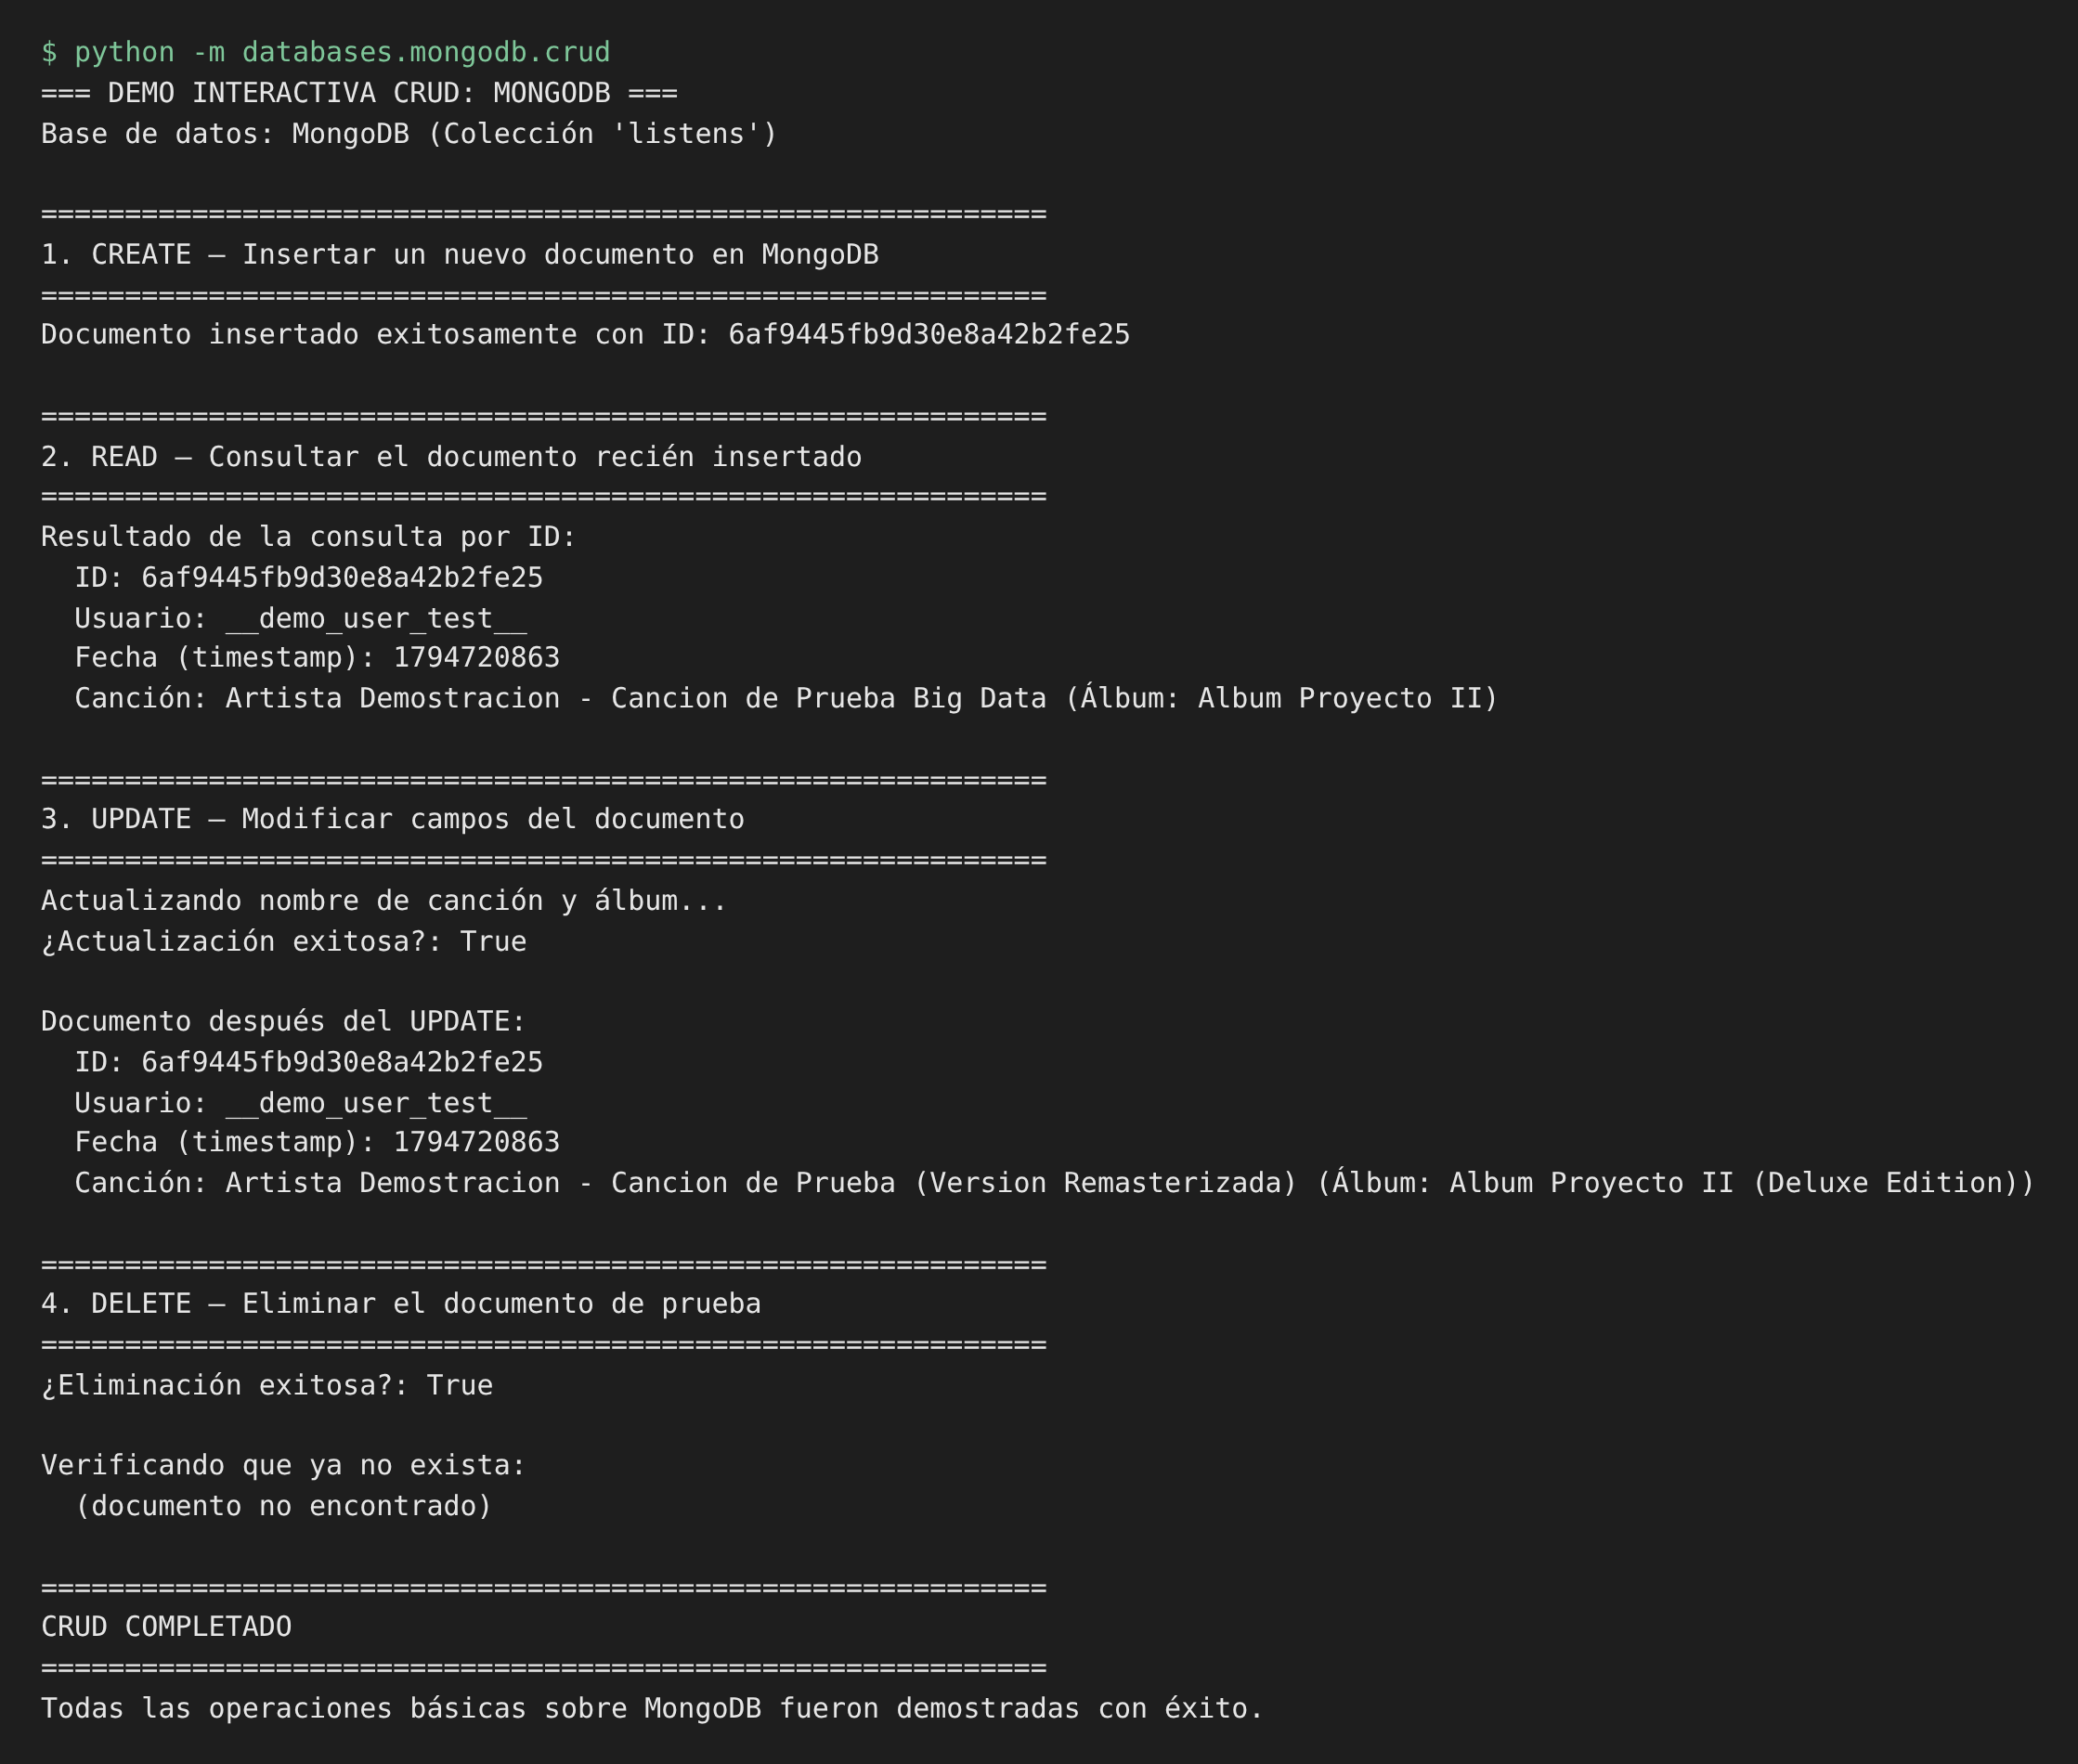
\includegraphics[width=\textwidth]{figuras/mongo_crud.png}
\end{figure}

El módulo incluye además una API REST con FastAPI sobre la misma colección, con documentación interactiva en Swagger. Las rutas bajo \code{/listens} cubren creación (\code{POST}), consulta por identificador y listado paginado (\code{GET}), actualización parcial y total (\code{PATCH} y \code{PUT}) y eliminación (\code{DELETE}), además de un resumen estadístico y un top de artistas. Cada solicitud pasa por la ruta, el modelo Pydantic que valida los campos (y responde 422 si son incorrectos antes de escribir en la base), un servicio que arma los filtros y un repositorio que ejecuta la operación con PyMongo. En la validación final se ejecutaron tres rondas completas de CRUD por HTTP contra la colección real y la cantidad de documentos quedó igual antes y después.

\subsection{Consultas y agregaciones}

\code{databases/mongodb/queries.py} define siete agregaciones: usuarios únicos, artistas únicos, top 5 de artistas, top 10 de canciones (agrupadas por artista y título), top 5 de usuarios, duración promedio de las pistas que traen \code{duration_ms} en \code{additional_info} y escuchas por día. La última convierte el \code{timestamp} a fecha y agrupa por día:

\begin{lstlisting}[language=Python]
"listens_by_day": [
    {"$match": {"timestamp": {"$type": "number", "$gte": 0, "$lte": 253402300799}}},
    {"$project": {"day": {"$dateToString": {"format": "%Y-%m-%d", "timezone": "UTC",
                  "date": {"$toDate": {"$multiply": ["$timestamp", 1000]}}}}}},
    {"$group": {"_id": "$day", "listen_count": {"$sum": 1}}},
    {"$sort": {"_id": 1}},
],
\end{lstlisting}

Estas agregaciones recorren la colección completa y sirven para exploración. Los indicadores que se consultan siempre, como las escuchas por día, se precalculan en Cassandra, que los sirve en milisegundos.

MongoDB guarda también la colección \code{kpi_runs}, donde Airflow deja un documento por corrida con los cinco KPIs, las métricas de seguimiento y la serie diaria reciente (sección~\ref{cap:kpis}).

\section{Modelo de datos de Cassandra}
\label{cap:cassandra}

Cassandra guarda las escuchas como serie temporal y las métricas agregadas por fecha que consume el dashboard \citep{cassandra}. MongoDB conserva el documento original y Neo4j las relaciones; aquí está lo que se consulta por tiempo y en volumen. El código está en \code{databases/cassandra/}.

\subsection{Por qué este diseño}

Son 4\,855\,809 escuchas y el DAG puede seguir agregando lotes, así que la base tiene que aceptar escrituras masivas. Las consultas del dashboard se conocen de antemano y son siempre las mismas: actividad por día, ranking del mes, evolución de un artista e historial de un usuario. En Cassandra eso se resuelve con una tabla por consulta (diseño \emph{query-first}), de modo que cada lectura va directo a una sola partición sin importar cuántos datos haya. Dentro de la partición, la clave de clustering deja las filas ordenadas por fecha. El costo es repetir datos entre tablas y no poder hacer consultas ad hoc: si aparece una pregunta nueva, hay que agregar otra tabla.

\subsection{Tablas}

El keyspace \code{music_dna} usa \code{SimpleStrategy} con factor de replicación 1, porque en desarrollo corremos un solo nodo. La tabla~\ref{tab:cassandra-tablas} resume las seis tablas.

\begin{table}[H]
\centering
\caption{Tablas del keyspace \code{music_dna}}
\label{tab:cassandra-tablas}
\small
\begin{tabularx}{\textwidth}{>{\raggedright\arraybackslash}p{3.3cm} >{\raggedright\arraybackslash}p{2.7cm} >{\raggedright\arraybackslash}p{3.2cm} Y}
\toprule
Tabla & Partición & Clustering & Consulta que responde \\
\midrule
\code{listens_by_user} & \code{(user_id, month)} & \code{listened_at DESC, listen_id} & Historial de un usuario en un mes \\
\code{daily_stats} & \code{year} & \code{day} & Serie diaria del año con sus KPIs \\
\code{top_artists_by_month} & \code{month} & \code{rank} & Top de artistas del mes, ya ordenado \\
\code{artist_monthly_listens} & \code{artist_name} & \code{month} & Evolución mensual de un artista \\
\code{user_daily_listens} & \code{user_id} & \code{day} & Actividad diaria de un usuario \\
\code{load_batches} & \code{batch_id} & -- & Lotes del archivo ya cargados \\
\bottomrule
\end{tabularx}
\end{table}

Las dos tablas principales se definen así en \code{schema.cql}:

\begin{lstlisting}[language=CQL]
CREATE TABLE IF NOT EXISTS music_dna.listens_by_user (
    user_id        bigint,
    month          text,
    listened_at    timestamp,
    listen_id      uuid,
    artist_name    text,
    track_name     text,
    release_name   text,
    recording_msid text,
    PRIMARY KEY ((user_id, month), listened_at, listen_id)
) WITH CLUSTERING ORDER BY (listened_at DESC, listen_id ASC);

CREATE TABLE IF NOT EXISTS music_dna.daily_stats (
    year             int,
    day              date,
    listens          bigint,
    active_users     int,
    listens_per_user double,
    growth_pct       double,
    PRIMARY KEY ((year), day)
);
\end{lstlisting}

Tres decisiones del modelo merecen explicación:

\begin{itemize}
  \item \code{listens_by_user} se particiona por usuario y mes, no solo por usuario. Así una partición no crece sin límite: la más grande del dataset tiene 14\,205 filas. Particionar solo por usuario habría acumulado todo el historial de los usuarios más activos en una sola partición.
  \item \code{top_artists_by_month} usa \code{rank} como clustering porque Cassandra solo ordena por columnas de clustering. El ranking se calcula al cargar y la consulta es un \texttt{SELECT ... LIMIT 10}.
  \item No se guarda \code{user_name}: con \code{user_id} alcanza y el dashboard no necesita exponer nombres de usuario.
\end{itemize}

\code{listen_id} es un UUID determinista (UUID versión 5) calculado a partir del usuario, el \code{timestamp}, el \code{recording_msid}, el artista y la canción. La misma escucha siempre genera el mismo id, y eso es lo que hace que recargar no duplique filas.

\subsection{Carga por lotes}

\code{databases/cassandra/loader.py} lee el JSONL en lotes de 500\,000 líneas. Para cada lote:

\begin{enumerate}
  \item Limpia cada línea: \code{user_id} y \code{timestamp} enteros, artista y canción no vacíos. Las líneas que no cumplen se cuentan como omitidas, y las escuchas repetidas dentro del lote (mismo \code{listen_id}) se descartan.
  \item Si el lote no está registrado en \code{load_batches}, escribe sus escuchas en \code{listens_by_user} y lo registra con sus conteos. El id del lote es el nombre del archivo más el rango de líneas, por ejemplo \code{listens_full.jsonl:1-500000}.
  \item Al terminar, recalcula las tablas agregadas (\code{daily_stats}, \code{top_artists_by_month}, \code{artist_monthly_listens} y \code{user_daily_listens}) con todas las escuchas cargadas hasta ese momento y las sobrescribe.
\end{enumerate}

Repetir la carga no duplica nada: las escuchas tienen id determinista y el \texttt{INSERT} sobrescribe la misma fila, los lotes registrados no se vuelven a escribir y los agregados se reemplazan en lugar de sumarse. La función \code{load_listens} acepta un máximo de lotes nuevos por ejecución, y eso es lo que usa Airflow para cargar un lote por corrida (sección~\ref{cap:airflow}). El tamaño de lote debe ser siempre el mismo, porque el id de cada lote depende de él.

Hicieron falta tres optimizaciones:

\begin{itemize}
  \item \textbf{BATCH por partición.} Las filas de la misma partición se envían juntas en un \texttt{UNLOGGED BATCH} de hasta 30 filas, que Cassandra aplica como una sola mutación. Fue unas 13 veces más rápido que una escritura por fila. Mezclar particiones en un mismo BATCH habría sido más lento.
  \item \textbf{Sin counters.} La primera versión usaba columnas \code{counter}, pero cada incremento lee antes de escribir, y con alrededor de un millón de claves artista--mes la carga se volvía cada vez más lenta. Además, si un reintento repite un lote, un counter suma dos veces. Recalcular y sobrescribir resultó más rápido y seguro.
  \item \textbf{\code{UNSET_VALUE} en lugar de \code{None}} para los campos opcionales, porque insertar \code{None} crea un tombstone (marca de borrado) por cada fila.
\end{itemize}

\subsection{Resultados de la carga completa}

Las mediciones se hicieron en un notebook con Windows~11, 20~GB de RAM y Cassandra~5.0 en Docker (un nodo, heap de 2~GB), cargando el archivo completo del incremental 2746 con las tablas vacías.

\begin{table}[H]
\centering
\caption{Tiempos de carga en Cassandra}
\label{tab:cassandra-tiempos}
\begin{tabularx}{\textwidth}{l Y}
\toprule
Etapa & Tiempo \\
\midrule
10 lotes de escuchas (lectura, limpieza y escritura) & 343~s, entre 7\,500 y 21\,600 filas por segundo según el lote \\
Recálculo de las tablas agregadas & 196~s \\
Total & 553~s (unos 9 minutos) \\
Segunda ejecución sin lotes nuevos & 439~s; los totales no cambian (4\,855\,809) \\
\bottomrule
\end{tabularx}
\end{table}

La segunda ejecución demuestra que la carga es idempotente, pero también muestra el costo del diseño: cada ejecución relee el archivo para recalcular los agregados, así que tarda unos 7 minutos aunque no haya lotes nuevos. Para el DAG es aceptable; si hiciera falta bajarlo, habría que recalcular solo los días y meses que tocó el lote nuevo.

\begin{table}[H]
\centering
\caption{Filas resultantes por tabla}
\label{tab:cassandra-filas}
\begin{tabularx}{\textwidth}{l Y}
\toprule
Tabla & Filas \\
\midrule
\code{listens_by_user} & 4\,855\,809 en 30\,315 particiones (la mayor, 14\,205 filas) \\
\code{artist_monthly_listens} & 961\,898 \\
\code{user_daily_listens} & 113\,827 \\
\code{daily_stats} & 7\,575 días, del 2005-02-13 al 2026-10-27 \\
\code{top_artists_by_month} & Hasta 50 artistas por cada uno de los 260 meses \\
\bottomrule
\end{tabularx}
\end{table}

El total se comprobó de tres formas independientes: la suma de \code{load_batches}, la suma de \code{daily_stats} y un \texttt{COUNT(*)} partición por partición en \code{listens_by_user}. Las tres dan 4\,855\,809, igual que \code{scripts/validate_dataset.py}, sin líneas omitidas ni duplicadas.

\subsection{Operaciones CRUD}

El CRUD está en \code{databases/cassandra/crud.py} y trabaja sobre \code{listens_by_user}, donde una fila es una escucha. Como \code{month} se calcula a partir de \code{listened_at}, para ubicar una escucha basta con \code{user_id}, \code{listened_at} y \code{listen_id}.

\begin{table}[H]
\centering
\caption{Operaciones CRUD en Cassandra}
\label{tab:cassandra-crud}
\begin{tabularx}{\textwidth}{l l Y}
\toprule
Operación & Función & CQL \\
\midrule
Insertar & \code{insert_listen} & \texttt{INSERT INTO listens\_by\_user (...) VALUES (...)} \\
Consultar una & \code{get_listen} & \texttt{SELECT * ... WHERE} con la clave primaria completa \\
Consultar el mes & \code{get_user_listens} & \texttt{SELECT * ... WHERE user\_id = ? AND month = ? LIMIT ?} \\
Actualizar & \code{update_listen} & \texttt{UPDATE listens\_by\_user SET track\_name = ?, release\_name = ?} con la clave \\
Eliminar & \code{delete_listen} & \texttt{DELETE FROM listens\_by\_user} con la clave \\
\bottomrule
\end{tabularx}
\end{table}

Dos detalles de Cassandra explican el código. Primero, \texttt{INSERT} y \texttt{UPDATE} son \emph{upserts}: un \texttt{UPDATE} sobre una fila que no existe la crea. Por eso \code{update_listen} y \code{delete_listen} leen la fila antes y devuelven \texttt{False} si no existe. Segundo, no usamos \texttt{IF EXISTS}. Lo probamos y fallaba: esas escrituras (transacciones ligeras) usan el reloj del servidor y las normales el del cliente. Con Docker en Windows, el \texttt{UPDATE ... IF EXISTS} respondía que se había aplicado, pero quedaba con un timestamp anterior al del \texttt{INSERT} y Cassandra conservaba el valor viejo.

La demostración (\code{python -m databases.cassandra.crud --step}) usa el usuario $-1$, que no existe en ListenBrainz: inserta una escucha, la lee, la corrige, la borra y comprueba que ya no está. Termina con una lectura real de las últimas escuchas de un usuario del dataset. El CRUD no modifica las tablas agregadas, que se recalculan en cada carga. La figura~\ref{fig:cassandra-crud} muestra los cuatro primeros pasos ejecutados contra el keyspace que dejó Airflow.

\begin{figure}[H]
\caption{Demostración del CRUD en Cassandra}
\label{fig:cassandra-crud}
\centering
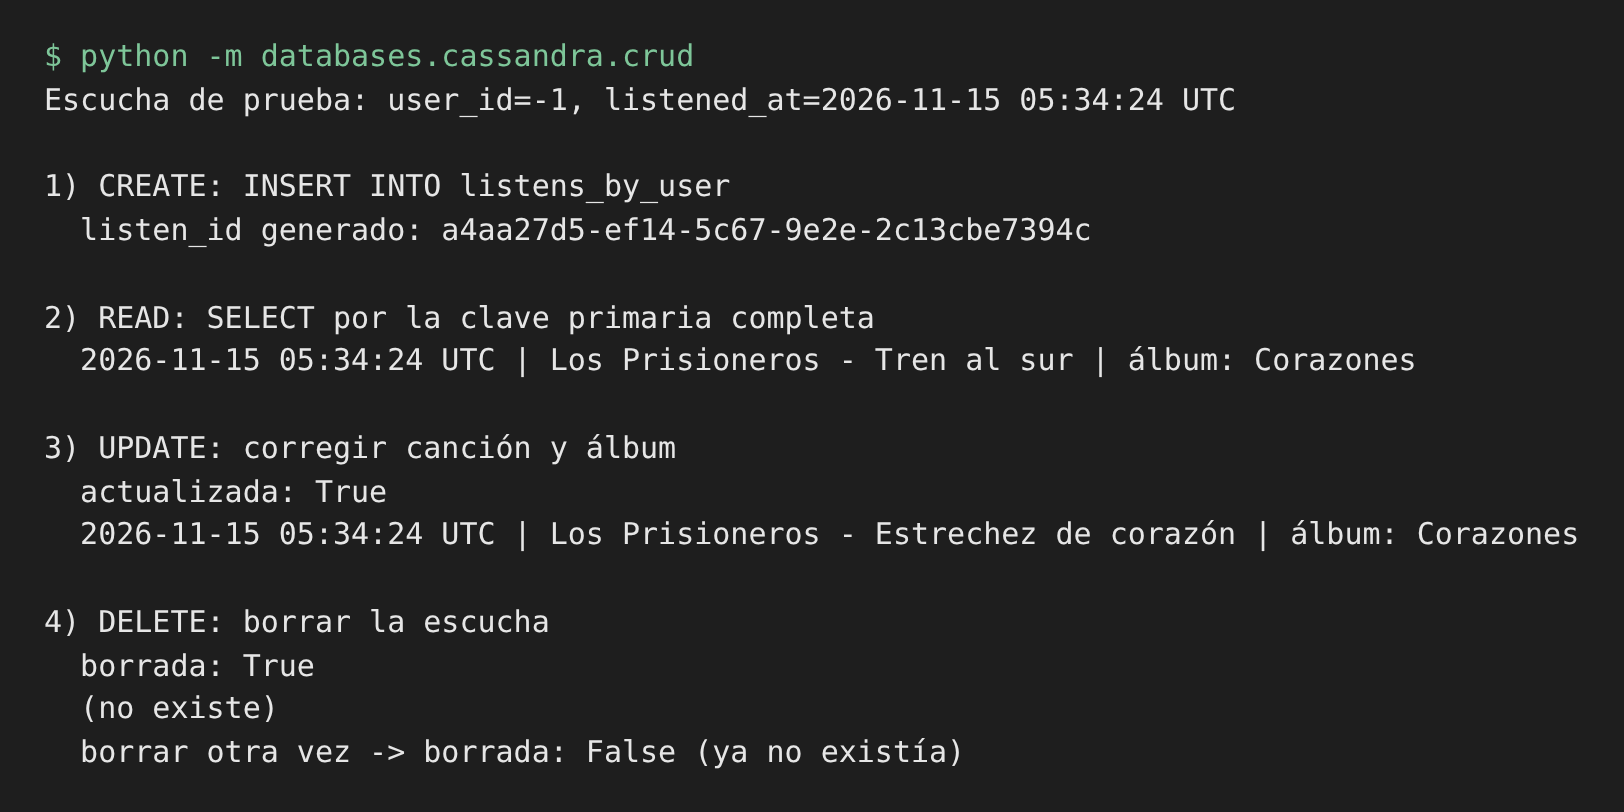
\includegraphics[width=0.9\textwidth]{figuras/cassandra_crud.png}
\nota{El quinto paso, la lectura de un usuario real, no se incluye para no publicar su identificador.}
\end{figure}

\subsection{Consultas}

\code{databases/cassandra/queries.py} tiene una función por consulta y todas devuelven listas de diccionarios, que el dashboard puede convertir directamente en tablas. Cada una lee una sola partición:

\begin{table}[H]
\centering
\caption{Consultas de Cassandra y tiempos medidos}
\label{tab:cassandra-consultas}
\begin{tabularx}{\textwidth}{l Y r}
\toprule
Función & Devuelve & Tiempo \\
\midrule
\code{get_daily_stats} & Escuchas, usuarios activos, escuchas por usuario y crecimiento de cada día del año & 6~ms \\
\code{get_top_artists} & Ranking del mes con escuchas y porcentaje del total & 11~ms \\
\code{get_artist_history} & Escuchas por mes de un artista & 16~ms \\
\code{get_user_activity} & Escuchas por día de un usuario & -- \\
\code{get_load_batches} & Lotes cargados, con filas cargadas y omitidas & -- \\
\bottomrule
\end{tabularx}
\nota{Tiempos medidos con el dataset completo: serie diaria de 2026, top 10 de octubre de 2026 e historial mensual de un artista. Leer las últimas 5 escuchas de la partición más grande de \code{listens_by_user} (14\,205 filas) tomó 14~ms.}
\end{table}

\subsection{Limitaciones}

El keyspace corre en un solo nodo con factor de replicación 1, que sirve para desarrollo pero no tolera caídas; en producción correspondería \code{NetworkTopologyStrategy} con factor 3. Los artistas se identifican por el nombre tal como viene en el dataset, así que homónimos y variantes de escritura cuentan por separado. Los agregados se recalculan desde el archivo, por lo que una escucha creada a mano con el CRUD no aparece en ellos. Por último, los duplicados se descartan dentro de cada lote; entre lotes \code{listens_by_user} no duplica (mismo id), pero los agregados contarían dos veces. En este dataset no hay duplicados: lo comprobamos sobre los 4\,855\,809 registros.

\section{Modelo de grafo en Neo4j}
\label{cap:neo4j}

Neo4j modela las relaciones entre usuarios, canciones y artistas; sobre ese grafo se calculan afinidades, comunidades, recomendaciones y la diversidad de escucha. El código está en \code{databases/neo4j/}, y el análisis de comunidades usa NetworkX.

\subsection{Nodos y relaciones}

La figura~\ref{fig:grafo} muestra el modelo y las tablas~\ref{tab:neo4j-nodos} y~\ref{tab:neo4j-relaciones} detallan las propiedades.

\begin{figure}[H]
\caption{Modelo de grafo}
\label{fig:grafo}
\centering
\begin{tikzpicture}[
  nodo/.style={draw, circle, minimum size=1.7cm, align=center, font=\small},
  rel/.style={-{Stealth[length=2.2mm]}, semithick},
  etiqueta/.style={font=\scriptsize, fill=white, inner sep=1.5pt}]
  \node[nodo] (u) {Usuario};
  \node[nodo, right=3.4cm of u] (c) {Canción};
  \node[nodo, below=2.2cm of c] (a) {Artista};
  \node[nodo, right=3.4cm of a] (com) {Comunidad};
  \node[nodo, below=2.2cm of u] (l) {Lote};
  \node[nodo, below=1.6cm of l] (an) {Análisis};
  \draw[rel] (u) -- node[etiqueta, above] {ESCUCHO} (c);
  \draw[rel] (c) -- node[etiqueta, right] {INTERPRETADA\_POR} (a);
  \draw[rel] (u) -- node[etiqueta, sloped, above] {ESCUCHA\_ARTISTA} (a);
  \draw[rel] (a) -- node[etiqueta, above] {PERTENECE\_A} (com);
  \draw[rel] (a) to[out=-60, in=-120, looseness=5] node[etiqueta, below] {AFIN\_A} (a);
  \draw[rel] (l) -- node[etiqueta, right] {ANALISIS\_ACTIVO} (an);
\end{tikzpicture}
\end{figure}

\begin{table}[H]
\centering
\caption{Nodos del grafo}
\label{tab:neo4j-nodos}
\begin{tabularx}{\textwidth}{l l Y}
\toprule
Etiqueta & Clave única & Otras propiedades \\
\midrule
\code{Usuario} & \code{id} (\code{user_id}) & -- \\
\code{Cancion} & \code{id} (\code{recording_msid}) & \code{titulo} \\
\code{Artista} & \code{nombre} & -- \\
\code{Lote} & \code{id} & \code{source_sha256}, \code{registros}, \code{estado} (cargando o completo) \\
\code{Analisis} & \code{id} & Parámetros, versión de NetworkX, indicadores del análisis y \code{estado} \\
\code{Comunidad} & \code{id} & \code{analisis}, \code{numero}, \code{artistas}, \code{audiencia}, \code{representantes} \\
\bottomrule
\end{tabularx}
\end{table}

\begin{table}[H]
\centering
\caption{Relaciones del grafo}
\label{tab:neo4j-relaciones}
\begin{tabularx}{\textwidth}{l l Y}
\toprule
Relación & Entre & Propiedades \\
\midrule
\code{ESCUCHO} & Usuario $\rightarrow$ Canción & \code{lote}, \code{cantidad}, \code{primera_escucha}, \code{ultima_escucha} \\
\code{INTERPRETADA_POR} & Canción $\rightarrow$ Artista & \code{lote} \\
\code{ESCUCHA_ARTISTA} & Usuario $\rightarrow$ Artista & \code{lote}, \code{cantidad}, \code{proporcion}, \code{primera_escucha}, \code{ultima_escucha} \\
\code{AFIN_A} & Artista -- Artista & \code{analisis}, \code{jaccard}, \code{usuarios_comunes}, audiencias de ambos artistas \\
\code{PERTENECE_A} & Artista $\rightarrow$ Comunidad & \code{analisis}, \code{puente} \\
\code{ANALISIS_ACTIVO} & Lote $\rightarrow$ Análisis & -- \\
\bottomrule
\end{tabularx}
\end{table}

Una relación \code{ESCUCHO} resume todas las reproducciones de un usuario a una canción (cantidad, primera y última fecha); \code{ESCUCHA_ARTISTA} hace lo mismo por artista y añade la proporción que representa en el historial del usuario. Esto reduce las 4,86 millones de escuchas a 1\,791\,408 relaciones \code{ESCUCHO} y 743\,531 \code{ESCUCHA_ARTISTA}. Las canciones se identifican por \code{recording_msid}, cada relación lleva su lote, y las claves únicas se garantizan con restricciones (\texttt{CREATE CONSTRAINT ... REQUIRE n.id IS UNIQUE}).

La figura~\ref{fig:neo4j-browser} muestra el grafo cargado en Neo4j Browser: Linkin Park, el artista con más oyentes (sección~\ref{cap:kpis}), y los 21 artistas con los que tiene una relación \code{AFIN_A}.

\begin{figure}[H]
\caption{Afinidades de Linkin Park en Neo4j Browser}
\label{fig:neo4j-browser}
\centering
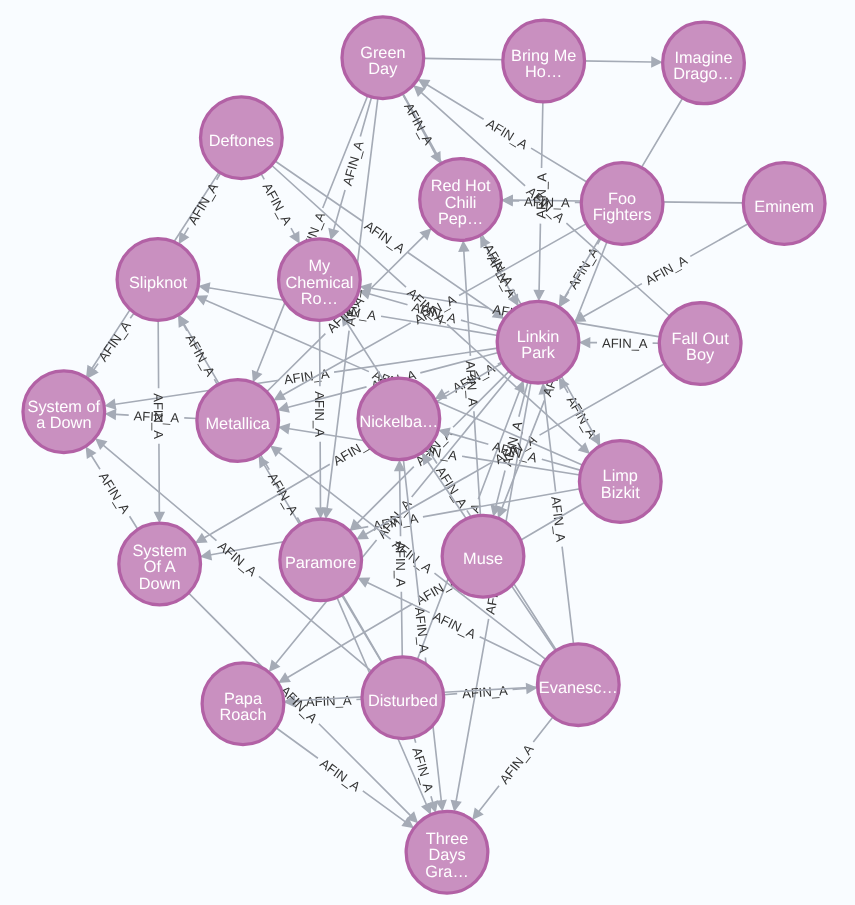
\includegraphics[width=0.62\textwidth]{figuras/neo4j_browser.png}
\end{figure}

\subsection{Carga}

La carga tiene dos etapas. \code{prepare} recorre el JSONL completo, valida cada fila, calcula el SHA-256 del archivo y agrega usuarios, canciones, artistas y pares usuario--canción y usuario--artista en un SQLite intermedio (\code{data/neo4j/prepared.sqlite}). Después \code{load_data} crea las restricciones, registra el nodo \code{Lote} en estado \code{cargando} y envía los datos en lotes de 1000 filas con \texttt{UNWIND} y \texttt{MERGE}, primero nodos y luego relaciones. Al final reconcilia que la cantidad de relaciones y la suma de \code{cantidad} coincidan con lo preparado, y solo entonces el lote pasa a \code{completo}. Como todo usa \texttt{MERGE}, repetir la carga no duplica nada.

\begin{lstlisting}[language=Cypher]
UNWIND $rows AS f
MATCH (u:Usuario {id:f.user}), (c:Cancion {id:f.track})
MERGE (u)-[r:ESCUCHO {lote:$dataset}]->(c)
SET r.cantidad=f.count, r.primera_escucha=f.first, r.ultima_escucha=f.last
\end{lstlisting}

La tabla~\ref{tab:neo4j-carga} resume la carga completa del incremental 2746.

\begin{table}[H]
\centering
\caption{Resultado de la carga completa en Neo4j}
\label{tab:neo4j-carga}
\begin{tabular}{l r}
\toprule
Medida & Resultado \\
\midrule
Escuchas procesadas & 4\,855\,809 \\
Usuarios & 26\,394 \\
Canciones (\code{recording_msid}) & 1\,420\,842 \\
Nombres de artista & 286\,291 \\
Relaciones \code{ESCUCHO} & 1\,791\,408 \\
Relaciones \code{ESCUCHA_ARTISTA} & 743\,531 \\
Relaciones \code{INTERPRETADA_POR} & 1\,424\,734 \\
Preparación en SQLite & 60,20~s \\
Carga en Neo4j & 174,90~s \\
Análisis y publicación & 3,64~s \\
\bottomrule
\end{tabular}
\end{table}

\subsection{Operaciones CRUD en Cypher}

\code{python -m databases.neo4j.crud --pause} trabaja sobre nodos \code{ManagedRecord} para no tocar el lote: crea un usuario y una canción de prueba, los une con \code{ESCUCHO}, actualiza \code{cantidad}, consulta el cambio y elimina relación y nodos con \texttt{DETACH DELETE}.

\begin{lstlisting}[language=Cypher]
MATCH (u:Usuario:ManagedRecord {id:-120012, grupo:$group})
MATCH (c:Cancion:ManagedRecord {id:'manual-track', grupo:$group})
MERGE (u)-[r:ESCUCHO {lote:$group}]->(c)
SET r.cantidad=1
RETURN type(r) AS relacion, r.cantidad AS cantidad
\end{lstlisting}

La figura~\ref{fig:neo4j-crud} muestra la demostración sobre el grafo completo.

\begin{figure}[H]
\caption{Demostración del CRUD en Neo4j}
\label{fig:neo4j-crud}
\centering
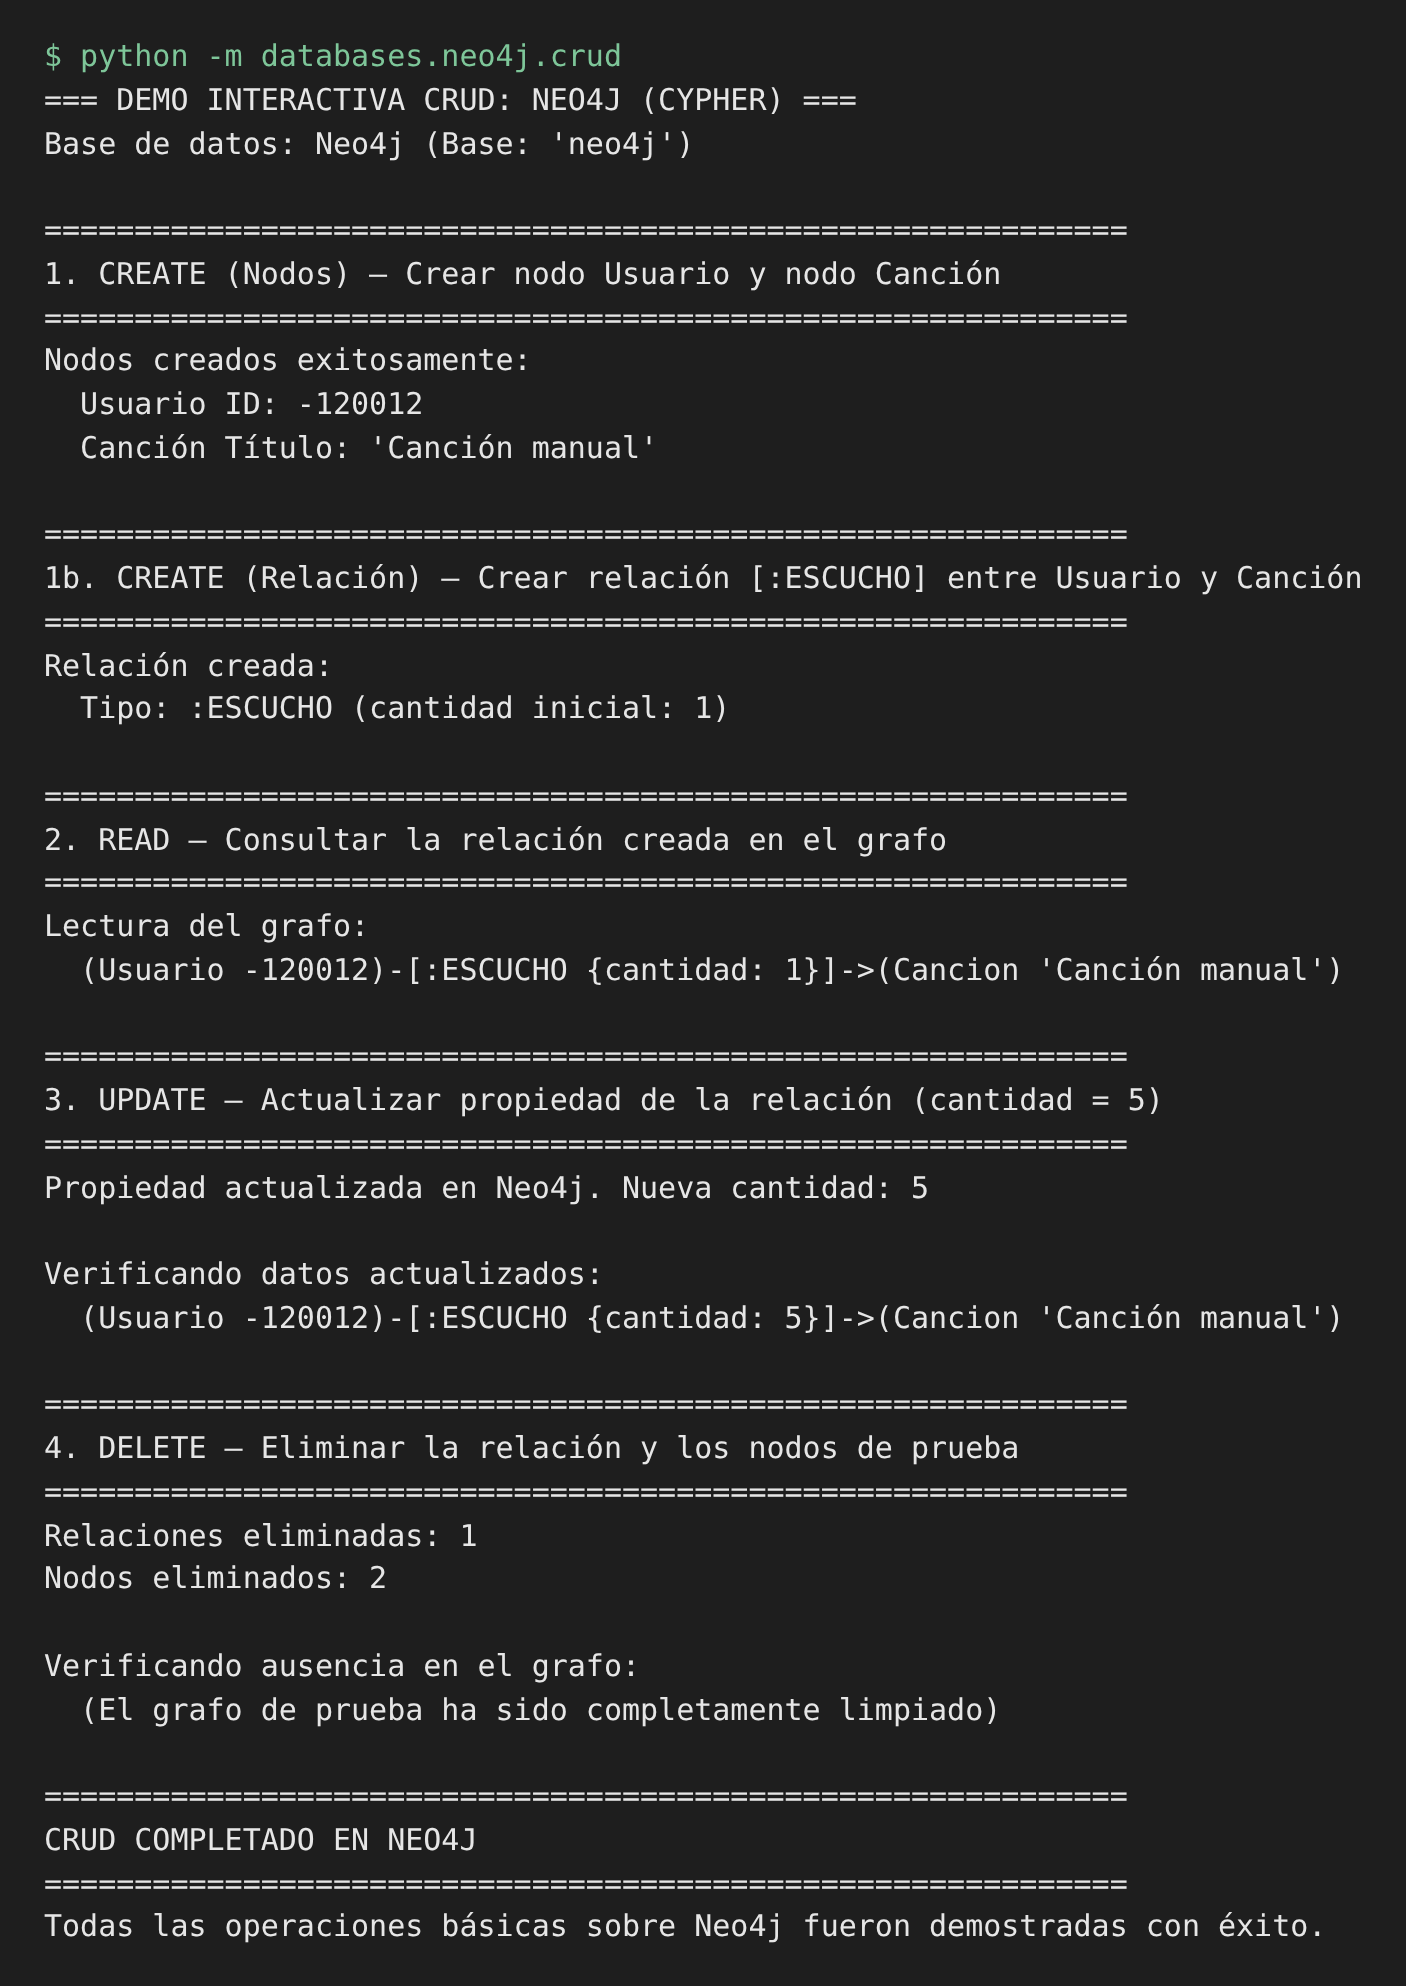
\includegraphics[width=0.68\textwidth]{figuras/neo4j_crud.png}
\end{figure}

\subsection{Afinidades y comunidades}

El análisis (\code{databases/neo4j/analyze.py}) usa los 500 artistas con más oyentes (al menos 20 cada uno). Para cada usuario se toman sus 20 artistas más escuchados y la audiencia $A(a)$ de un artista es el conjunto de usuarios que lo tienen en ese top. La afinidad entre dos artistas es el índice de Jaccard de sus audiencias:

\[
J(a,b) = \frac{|A(a) \cap A(b)|}{|A(a) \cup A(b)|}
\]

Se conservan los pares con al menos 10 usuarios en común y $J \geq 0{,}05$, y los 10 vecinos más afines de cada artista. Sobre ese grafo ponderado se detectan comunidades con Louvain (resolución 1, semilla 42) y se guardan en Neo4j las relaciones \code{AFIN_A}, las comunidades y los indicadores.

El coeficiente puente de cada artista mide cómo se reparten sus conexiones entre comunidades. Si $w_{a,c}$ es la suma de los pesos de Jaccard de las aristas de $a$ hacia artistas de la comunidad $c$ y $W_a$ la suma total:

\[
\text{puente}(a) = 1 - \sum_{c} \left( \frac{w_{a,c}}{W_a} \right)^2
\]

Vale 0 si todas sus conexiones están en una comunidad y crece al repartirse. La diversidad de un usuario es la entropía de Shannon normalizada de sus escuchas entre comunidades, con $p_{u,c}$ la fracción de sus escuchas clasificadas en la comunidad $c$ y $k_u$ el número de comunidades que escucha:

\[
D(u) = -\frac{\sum_{c} p_{u,c} \ln p_{u,c}}{\ln k_u}
\]

con $D(u) = 0$ si escucha una sola comunidad. Las tablas~\ref{tab:neo4j-analisis} y~\ref{tab:neo4j-comunidades} resumen el resultado.

\begin{table}[H]
\centering
\caption{Resultado del análisis de afinidades y comunidades}
\label{tab:neo4j-analisis}
\begin{tabular}{l r}
\toprule
Medida & Resultado \\
\midrule
Artistas seleccionados & 500 \\
Artistas conectados / aislados & 425 / 75 \\
Afinidades retenidas & 1\,553 \\
Comunidades & 13 \\
Modularidad ponderada & 0,782546 \\
Usuarios con recomendaciones & 16\,372 \\
Cobertura sobre los usuarios del lote & 62,03~\% \\
Escuchas clasificadas en comunidades & 1\,153\,631 (23,76~\%) \\
Diversidad media de usuarios clasificados & 0,416633 \\
\bottomrule
\end{tabular}
\end{table}

\begin{table}[H]
\centering
\caption{Comunidades detectadas}
\label{tab:neo4j-comunidades}
\begin{tabular}{r r r l}
\toprule
Comunidad & Artistas & Audiencia & Primeros representantes \\
\midrule
1 & 39 & 3\,556 & Travis Scott, Kendrick Lamar, Future \\
2 & 86 & 6\,585 & Linkin Park, Three Days Grace, Korn \\
3 & 84 & 6\,348 & Ariana Grande, Charli xcx, Taylor Swift \\
4 & 85 & 5\,545 & The Rolling Stones, Metallica, AC/DC \\
5 & 15 & 1\,611 & Ado, YOASOBI, Eve \\
6 & 17 & 1\,217 & Jin, Jimin, j-hope \\
7 & 11 & 1\,219 & Moby, Massive Attack, Air \\
8 & 13 & 1\,131 & ILLIT, LE SSERAFIM, aespa \\
9 & 65 & 6\,310 & Malcolm Todd, The Smiths, Radiohead \\
10 & 2 & 209 & Bill Withers, Marvin Gaye \\
11 & 2 & 246 & Crystal Castles, Grimes \\
12 & 2 & 242 & Hans Zimmer, Max Richter \\
13 & 4 & 533 & Royal Blood, The Black Keys, Nothing But Thieves \\
\bottomrule
\end{tabular}
\end{table}

Las comunidades agrupan artistas cercanos (rap estadounidense, metal y rock alternativo, pop, rock clásico, J-pop, solistas de BTS, música electrónica, K-pop); sus números identifican una partición concreta. Los representantes son los artistas con mayor grado ponderado de cada comunidad.

\subsection{Recomendaciones y consultas}

La recomendación para un usuario suma, por cada artista que aún no escucha, su afinidad con los artistas que sí escucha, ponderada por el peso de cada uno en su historial:

\[
\text{puntaje}(u, n) = \sum_{k \in K(u)} \text{proporcion}(u,k) \cdot J(k,n)
\]

donde $K(u)$ son los artistas que escucha $u$. La consulta devuelve también la evidencia (artista conocido y Jaccard):

\begin{lstlisting}[language=Cypher]
MATCH (l:Lote {id:$dataset, estado:'completo'})-[:ANALISIS_ACTIVO]->(an:Analisis)
MATCH (u:Usuario {id:$user})-[p:ESCUCHA_ARTISTA {lote:l.id}]->(conocido:Artista)
MATCH (conocido)-[f:AFIN_A {analisis:an.id}]-(nuevo:Artista)
WHERE NOT EXISTS { MATCH (u)-[:ESCUCHA_ARTISTA {lote:l.id}]->(nuevo) }
WITH nuevo, sum(p.proporcion * f.jaccard) AS puntaje,
     collect({artista_conocido:conocido.nombre, jaccard:f.jaccard}) AS evidencia
RETURN nuevo.nombre AS artista, puntaje, evidencia
ORDER BY puntaje DESC LIMIT $limit
\end{lstlisting}

Por ejemplo, una escucha de Motörhead lleva a recomendar Judas Priest: comparten 17 oyentes, con Jaccard 0,091892 y puntaje 0,032819. La consulta de canciones devuelve \emph{Breaking the Law}, y el camino más corto entre ambos artistas tiene un salto. Radiohead aparece con coeficiente puente 0,634146.

\code{python -m databases.neo4j.queries} ejecuta el resto de consultas: artistas con más oyentes, canciones de un artista, escuchas de un usuario, búsqueda por texto, totales del lote, recomendación de canciones, comunidades, artistas puente, diversidad e indicadores del análisis. La de artistas con más oyentes la usa Airflow para el KPI 5 (sección~\ref{cap:kpis}).

\section{Explicación del DAG de Airflow}
\label{cap:airflow}

El DAG \code{music_dna_pipeline} automatiza todo el flujo del proyecto: toma el volcado de ListenBrainz, lo valida, lo carga en MongoDB, Cassandra y Neo4j y al final calcula los KPIs que lee el dashboard \citep{airflow}. Se ejecuta todos los días (\code{@daily}) y en cada corrida agrega un bloque nuevo de escuchas, así se simula que los datos llegan de forma incremental.

El DAG no tiene lógica propia de carga ni de análisis. Cada tarea llama a las funciones que ya están en \code{databases/}, las mismas que se usan por consola, de modo que lo que se probó por separado en cada base es exactamente lo que corre en Airflow. El código está en \code{airflow/dags/music_dna_dag.py}.

\subsection{Airflow dentro del stack de Docker}

Airflow se agregó al \code{docker-compose.yml} de la raíz con cuatro servicios: \code{postgres} como base de metadatos (corridas, estados de tareas y XCom), \code{airflow-init}, que corre una sola vez para migrar esa base y crear el usuario administrador, \code{airflow-webserver} con la interfaz en el puerto 8080 y \code{airflow-scheduler}, que programa las corridas y ejecuta las tareas. La configuración común está en un bloque \code{x-airflow-common} para no repetirla en cada servicio.

La imagen propia (\code{airflow/Dockerfile}) parte de \code{apache/airflow:2.10.5-python3.11}. Le agrega \texttt{curl}, \texttt{zstd} y \texttt{tar}, que necesita el script de descarga, y los paquetes del pipeline: pymongo, pydantic, cassandra-driver, neo4j, networkx, python-dotenv y pytz. Se instalan con el archivo de constraints oficial de Airflow para no cambiar las versiones de sus propias dependencias. Streamlit y FastAPI no se instalan porque no corren dentro de Airflow.

Usamos \code{LocalExecutor}: las tareas corren como procesos dentro del contenedor del scheduler y pueden ejecutarse en paralelo. Para una sola máquina alcanza; Celery o Kubernetes harían falta recién con varios nodos de trabajo.

Dentro de los contenedores se montan \code{airflow/dags}, \code{databases}, \code{scripts} y \code{data} en \code{/opt/airflow/}, con \code{PYTHONPATH=/opt/airflow}. Así funcionan los imports \code{databases.mongodb}, \code{databases.cassandra} y \code{databases.neo4j}, y también las rutas de Neo4j, que se calculan desde la raíz del proyecto. Las bases se alcanzan por su nombre de servicio en la red de Docker (\code{mongodb://mongodb:27017/}, \code{CASSANDRA_HOSTS=cassandra}, \code{bolt://neo4j:7687}), no por \code{localhost}. Los servicios de Airflow esperan con \texttt{depends\_on} y \texttt{condition: service\_healthy} a que postgres y las tres bases respondan su healthcheck.

\subsection{Estructura del DAG}

\begin{table}[H]
\centering
\caption{Configuración del DAG}
\label{tab:dag-config}
\begin{tabularx}{\textwidth}{l Y}
\toprule
Parámetro & Valor \\
\midrule
\code{dag_id} & \code{music_dna_pipeline} \\
Programación & \code{@daily}, desde el 1 de noviembre de 2026, con \code{catchup=False} \\
Corridas simultáneas & \code{max_active_runs=1} \\
Reintentos & 2 por tarea, con 5 minutos de espera \\
Tiempo máximo por tarea & 2 horas \\
Dataset & \code{/opt/airflow/data/processed/listens_full.jsonl} \\
\bottomrule
\end{tabularx}
\end{table}

\code{catchup=False} evita que al activar el DAG se lancen corridas atrasadas por cada día desde la fecha de inicio. \code{max_active_runs=1} es necesario porque cada corrida continúa donde quedó la anterior: dos corridas a la vez intentarían cargar el mismo bloque. Las seis tareas y sus dependencias se muestran en la figura~\ref{fig:dag}.

\begin{figure}[H]
\caption{Tareas del DAG \code{music_dna_pipeline} y sus dependencias}
\label{fig:dag}
\centering
\begin{tikzpicture}[
  tarea/.style={draw, rounded corners=2pt, align=center, minimum height=0.9cm, minimum width=2.7cm, font=\small\ttfamily},
  flecha/.style={-{Stealth[length=2.2mm]}, semithick}]
  \node[tarea] (ext) {extraer\_datos};
  \node[tarea, right=0.6cm of ext] (val) {validar\_y\_limpiar};
  \node[tarea, right=0.9cm of val] (cas) {cargar\_cassandra};
  \node[tarea, above=0.35cm of cas] (mon) {cargar\_mongodb};
  \node[tarea, below=0.35cm of cas] (neo) {cargar\_neo4j};
  \node[tarea, right=0.9cm of cas] (kpi) {generar\_kpis};
  \draw[flecha] (ext) -- (val);
  \draw[flecha] (val.east) -- (mon.west);
  \draw[flecha] (val) -- (cas);
  \draw[flecha] (val.east) -- (neo.west);
  \draw[flecha] (mon.east) -- (kpi.west);
  \draw[flecha] (cas) -- (kpi);
  \draw[flecha] (neo.east) -- (kpi.west);
\end{tikzpicture}
\nota{En el código la dependencia se expresa como \code{extraer_datos >> validar_y_limpiar >> [cargar_mongodb, cargar_cassandra, cargar_neo4j] >> generar_kpis}.}
\end{figure}

Las tareas usan la API TaskFlow de Airflow: cada una es una función decorada con \code{@task}, y las dependencias salen de pasar el resultado de una tarea como argumento de la siguiente. Los imports de \code{databases} van dentro de cada tarea para que el scheduler pueda leer el archivo del DAG rápido aunque una base no esté disponible. El final del archivo arma el flujo:

\begin{lstlisting}[language=Python]
extraccion = extraer_datos()
validacion = validar_y_limpiar(extraccion)
generar_kpis(cargar_mongodb(validacion), cargar_cassandra(validacion), cargar_neo4j(validacion))
\end{lstlisting}

Cada tarea devuelve un diccionario pequeño (conteos, rutas, banderas) que queda como XCom y se puede revisar en la interfaz. Los datos grandes nunca pasan por XCom: las tareas se comunican a través del archivo y de las bases. Los tamaños de lote se configuran como variables de Airflow, desde la interfaz y sin tocar el código:

\begin{table}[H]
\centering
\caption{Variables de Airflow del pipeline}
\label{tab:dag-variables}
\begin{tabularx}{\textwidth}{l r Y}
\toprule
Variable & Por defecto & Uso \\
\midrule
\code{music_dna_mongo_limit} & 100000 & Documentos nuevos por corrida en MongoDB \\
\code{music_dna_mongo_batch_size} & 2000 & Documentos por \code{insert_many} \\
\code{music_dna_cassandra_batch_size} & 500000 & Líneas por lote de Cassandra; no conviene cambiarlo después de la primera carga \\
\bottomrule
\end{tabularx}
\end{table}

\subsection{Las seis tareas}

\subsubsection{\texorpdfstring{\texttt{extraer\_datos}}{extraer\_datos}}

Si el JSONL ya está en \code{data/processed/}, lo reporta y no descarga nada. Si no, ejecuta \code{bash scripts/download_dataset.sh --extract}, que baja el incremental 2746 de MetaBrainz \citep{incremental2746}, verifica el SHA-256 oficial y extrae el archivo de escuchas. Devuelve la ruta, el tamaño y la cantidad de líneas. Va primero porque todas las demás tareas leen ese archivo.

\subsubsection{\texorpdfstring{\texttt{validar\_y\_limpiar}}{validar\_y\_limpiar}}

Ejecuta \code{scripts/validate_dataset.py --file <ruta>}, que recorre el archivo en streaming y comprueba que cada línea sea un objeto JSON con los campos obligatorios y que haya exactamente 4\,855\,809 registros (sección~\ref{cap:dataset}). Si el script termina con error, la tarea falla y las cargas no se ejecutan. Además deja \code{data/airflow/validacion.json} con los registros leídos, válidos e inválidos y el rango de fechas.

Esta tarea es un control de calidad del archivo completo. La limpieza registro por registro la hace cada loader al cargar, porque cada base necesita cosas distintas: MongoDB valida el esquema con Pydantic y descarta duplicados por la huella SHA-256 del documento; Cassandra exige \code{user_id} y \code{timestamp} enteros y artista y canción no vacíos, y descarta duplicados dentro del lote por su id determinista; Neo4j exige además \code{recording_msid}. Repetir esa lógica en Airflow solo duplicaría código.

\subsubsection{\texorpdfstring{\texttt{cargar\_mongodb}}{cargar\_mongodb}}

Llama a \code{load_to_mongodb} con \code{limit=100000}, \code{batch_size=2000} y el estado en \code{data/airflow/mongo_state.sqlite3}. En ese SQLite el loader guarda en qué byte del archivo quedó y las huellas de los documentos ya insertados, así que cada corrida sigue desde donde terminó la anterior y no inserta dos veces el mismo documento.

\subsubsection{\texorpdfstring{\texttt{cargar\_cassandra}}{cargar\_cassandra}}

Primero crea el keyspace y las tablas con \code{create_schema}; como son sentencias \texttt{CREATE ... IF NOT EXISTS}, no pasa nada si ya existen. Después llama a \code{load_listens} con \code{max_batches=1}: carga un lote nuevo de 500\,000 líneas en \code{listens_by_user}, lo registra en \code{load_batches} y recalcula las tablas agregadas con todo lo cargado hasta ese momento. La sesión se cierra siempre, aunque la carga falle:

\begin{lstlisting}[language=Python]
session = get_session(keyspace=None)
try:
    create_schema(session)  # CREATE ... IF NOT EXISTS, se puede repetir
    session.set_keyspace(KEYSPACE)
    summary = load_listens(session, DATASET_PATH, batch_size=batch_size, max_batches=1)
finally:
    session.cluster.shutdown()
\end{lstlisting}

\subsubsection{\texorpdfstring{\texttt{cargar\_neo4j}}{cargar\_neo4j}}

Sigue el mismo flujo que la carga por consola de Neo4j. Si no existe \code{data/neo4j/prepared.sqlite}, llama a \code{prepare}. Luego consulta el nodo \code{Lote} del dataset: si su estado es \code{completo}, lo registra en el log y no recarga; si no, ejecuta \code{load_data}. Al final cuenta usuarios, canciones, relaciones y escuchas del lote, y devuelve esos totales.

Las tres cargas dependen solo de la validación y no entre sí, por eso van en paralelo. Si una falla, las otras dos terminan igual, y al reintentar solo se repite la que falló.

\subsubsection{\texorpdfstring{\texttt{generar\_kpis}}{generar\_kpis}}

Espera a las tres cargas. Ejecuta el análisis de afinidades y comunidades de Neo4j, que guarda su resultado en el grafo y en \code{data/neo4j/analysis.json}. Luego consulta Cassandra con \code{get_daily_stats}, \code{get_top_artists} y \code{get_load_batches}, busca en Neo4j el artista con más oyentes y cuenta los documentos de MongoDB. Con eso arma los cinco KPIs (sección~\ref{cap:kpis}) y guarda un snapshot con el identificador de la corrida y la fecha en la colección \code{kpi_runs} de MongoDB y en \code{data/airflow/kpis_latest.json}.

\subsection{Carga incremental simulada}

El dataset es un solo archivo, así que la llegada de datos nuevos se simula cargando una parte en cada corrida:

\begin{table}[H]
\centering
\caption{Lo que agrega cada corrida del DAG}
\label{tab:dag-incremental}
\begin{tabularx}{\textwidth}{l Y Y}
\toprule
Base & Qué agrega cada corrida & Corridas para cubrir el archivo \\
\midrule
MongoDB & 100\,000 documentos nuevos, desde el byte donde quedó la anterior & 40, por el tope de 4\,000\,000 documentos del loader \\
Cassandra & 1 lote de 500\,000 líneas y recálculo de agregados & 10 \\
Neo4j & Nada después de la primera carga completa & 1 \\
\bottomrule
\end{tabularx}
\end{table}

Para que MongoDB fuera incremental hubo que corregir \code{load_to_mongodb}, como se explica en la sección~\ref{cap:mongodb}: el total objetivo pasó a ser lo que ya hay en la colección más \code{limit}. En Cassandra el id de cada lote es \code{listens_full.jsonl:<primera línea>-<última línea>}, por eso el tamaño de lote tiene que ser siempre el mismo; si cambiara, los ids no coincidirían con los ya registrados y los agregados contarían dos veces.

Como los KPIs se recalculan en cada corrida con lo que hay en las bases, cambian a medida que crece Cassandra. Cuando se terminan los lotes, las corridas siguen funcionando, pero los valores se estabilizan.

\subsection{Por qué Neo4j se carga una sola vez}

El loader de Neo4j no está pensado para cargar por partes. \code{prepare} exige el archivo completo (falla si no tiene 4\,855\,809 filas) y guarda el SHA-256 del archivo en el nodo \code{Lote}. Las relaciones \code{ESCUCHO} y \code{ESCUCHA_ARTISTA} guardan la cantidad total de escuchas de cada par usuario--canción y usuario--artista, y la proporción de cada artista en el historial del usuario. Esos valores se calculan sobre todo el lote: cargar por partes obligaría a sumar sobre lo ya cargado y recalcular las proporciones, es decir, escribir otro loader.

Además el grafo responde preguntas de relaciones (afinidades, comunidades, recomendaciones) que no ganan nada con ver el lote a medias. Por eso la tarea carga el grafo completo la primera vez y en las siguientes solo comprueba que el lote esté completo. Como la carga usa \texttt{MERGE}, aunque se repitiera no duplicaría nodos ni relaciones.

\subsection{Idempotencia y reintentos}

Cada tarea se puede repetir sin dejar datos duplicados, y eso es lo que hace seguros los dos reintentos automáticos:

\begin{table}[H]
\centering
\caption{Comportamiento de cada tarea al repetirse}
\label{tab:dag-idempotencia}
\begin{tabularx}{\textwidth}{l Y}
\toprule
Tarea & Qué pasa si se repite \\
\midrule
\code{extraer_datos} & Si el archivo ya está, no descarga. La extracción escribe a un \code{.part} y lo renombra al final, nunca deja un archivo a medias \\
\code{validar_y_limpiar} & Solo lee el archivo y sobrescribe el reporte \\
\code{cargar_mongodb} & Sigue desde el último checkpoint; los documentos tienen un \code{_id} derivado de su huella, así que un reintento no los duplica \\
\code{cargar_cassandra} & Los lotes registrados en \code{load_batches} se saltan, las escuchas tienen id determinista y los agregados se reemplazan, no se suman \\
\code{cargar_neo4j} & Si el lote está completo, no hace nada; si quedó en estado \code{cargando}, \code{load_data} vuelve a correr con \texttt{MERGE} \\
\code{generar_kpis} & El análisis borra y vuelve a crear sus propias afinidades y comunidades; el snapshot se guarda con \code{replace_one} usando el identificador de la corrida como \code{_id} \\
\bottomrule
\end{tabularx}
\end{table}

Si una corrida de MongoDB falla en medio de un lote, el checkpoint queda en el último lote confirmado y las huellas se reconstruyen leyendo la colección al empezar, así que lo que alcanzó a insertarse no se vuelve a insertar.

\subsection{Cómo se ejecuta}

Con el stack levantado (\texttt{docker compose build} y \texttt{docker compose up -d}), la interfaz de Airflow queda en \url{http://localhost:8080}. El DAG aparece pausado: se activa con el interruptor y se lanza con el botón de ejecución, o se deja que el scheduler lo dispare una vez al día. También se puede correr completo desde la terminal:

\begin{lstlisting}[language=bash]
docker compose exec airflow-scheduler airflow dags list-import-errors
docker compose exec airflow-scheduler airflow dags test music_dna_pipeline
\end{lstlisting}

Si el dataset no está en \code{data/processed/}, la primera tarea lo descarga. El resultado queda en \code{data/airflow/kpis_latest.json} y en la colección \code{kpi_runs}.

\section{KPIs implementados}
\label{cap:kpis}

Definimos cinco indicadores. Los cuatro primeros salen de las tablas agregadas de Cassandra y el quinto del grafo de Neo4j. Los calcula la tarea \code{generar_kpis} del DAG en cada corrida (sección~\ref{cap:airflow}), así que se actualizan a medida que se cargan lotes nuevos.

\subsection{Día de referencia}

Los indicadores diarios se calculan sobre un día de referencia $d^{*}$, que es el penúltimo día de la tabla \code{daily_stats}. El último día se descarta porque el volcado se cortó el 27 de octubre de 2026 a las 00:01 y ese día tiene solo 4 escuchas: usarlo daría un crecimiento de $-100\,\%$ que no dice nada sobre los usuarios. El mes de referencia $m^{*}$ es el mes de $d^{*}$.

En las fórmulas, $E(d)$ es la cantidad de escuchas con fecha $d$ (en UTC) y $U(d)$ la cantidad de usuarios distintos con al menos una escucha ese día. Ambos valores están precalculados en \code{daily_stats}.

Hay que leer todos los valores con una advertencia: el dataset es un lote de ingesta. Los indicadores describen lo que los usuarios enviaron a ListenBrainz en ese periodo, no la popularidad general de los artistas ni el comportamiento de toda la plataforma.

\subsection{KPI 1: escuchas procesadas por día}

\textit{Definición.} Cantidad de escuchas cargadas con fecha igual al día de referencia.

\textit{Fórmula.}
\[
\text{KPI}_1 = E(d^{*})
\]

\textit{Interpretación.} Mide el volumen que procesa el pipeline. Una caída fuerte respecto a los días anteriores indica un día con menos datos de lo normal, por ejemplo un corte del volcado o una falla de la fuente. Con el archivo completo cargado, el 26 de octubre tiene 1\,359\,824 escuchas, el 28~\% de todo el dataset, lo que muestra cuánto se concentra la ingesta en los últimos días del incremental.

\subsection{KPI 2: crecimiento diario de escuchas}

\textit{Definición.} Variación porcentual de las escuchas del día de referencia respecto al día anterior.

\textit{Fórmula.}
\[
\text{KPI}_2 = \frac{E(d^{*}) - E(d^{*}-1)}{E(d^{*}-1)} \times 100
\]
El valor queda vacío si $E(d^{*}-1) = 0$.

\textit{Interpretación.} Muestra la tendencia de corto plazo. En este dataset tiene saltos muy grandes: con el archivo completo, el 26 de octubre crece $+3\,364\,\%$ respecto al día anterior. Un salto así refleja un cambio en la ingesta (muchos usuarios enviando su historial en esos días), no que la gente haya escuchado treinta veces más música.

\subsection{KPI 3: escuchas promedio por usuario activo}

\textit{Definición.} Promedio de escuchas de los usuarios que escucharon algo el día de referencia.

\textit{Fórmula.}
\[
\text{KPI}_3 = \frac{E(d^{*})}{U(d^{*})}
\]

\textit{Interpretación.} Separa intensidad de alcance. Si suben las escuchas pero no los usuarios activos, los mismos usuarios están escuchando más; si suben ambos en la misma proporción, hay más usuarios con un comportamiento parecido. Con el archivo completo, el 26 de octubre tiene 1\,359\,824 escuchas de 26\,020 usuarios, unas 52,3 escuchas por usuario activo.

\subsection{KPI 4: participación del artista líder del mes}

\textit{Definición.} Porcentaje de las escuchas del mes de referencia que corresponde al artista más escuchado de ese mes.

\textit{Fórmula.} Si $E_{a}(m)$ son las escuchas del artista $a$ en el mes $m$ y $a_1$ es el artista en el primer puesto del ranking:
\[
\text{KPI}_4 = \frac{E_{a_1}(m^{*})}{\sum_{a} E_{a}(m^{*})} \times 100
\]
El valor se lee de \code{share_pct} en la fila con \code{rank = 1} de \code{top_artists_by_month}, que se calcula al cargar sobre todas las escuchas del mes.

\textit{Interpretación.} Mide concentración. Un valor alto indica que un solo artista domina la escucha del mes; uno bajo, que la escucha está repartida entre muchos artistas. Con el archivo completo, BTS concentra el 12,65~\% de las escuchas de octubre de 2026, un valor alto si se considera que el lote tiene 286\,291 nombres de artista distintos.

\subsection{KPI 5: entidad con más conexiones en el grafo}

\textit{Definición.} Artista con más usuarios distintos conectados a él en el grafo, es decir, con más oyentes.

\textit{Fórmula.} Si $C(a)$ es la cantidad de usuarios con una relación \code{ESCUCHA_ARTISTA} hacia el artista $a$:
\[
C(a) = \left|\{\, u : (u)\text{-[:ESCUCHA\_ARTISTA]}\rightarrow(a) \,\}\right|, \qquad \text{KPI}_5 = \max_{a} C(a)
\]
El indicador reporta el artista que alcanza el máximo y su valor $C(a)$. Se obtiene con la consulta de artistas con más oyentes del módulo de Neo4j.

\textit{Interpretación.} Es el grado de entrada del artista en el grafo usuario--artista: cuántos usuarios distintos lo escuchan, sin importar cuántas veces. Mide alcance y no volumen, y por eso complementa al KPI 4: un artista puede tener muchas escuchas concentradas en pocos fans y otro, menos escuchas repartidas entre mucha gente.

\subsection{Métricas de seguimiento}

Además de los cinco KPIs, cada snapshot guarda métricas que sirven para seguir el estado del pipeline: el total acumulado de documentos en MongoDB y los insertados en la corrida, los lotes y escuchas cargados en Cassandra, los usuarios, canciones y escuchas del grafo, y los indicadores del análisis de Neo4j (cantidad de comunidades, modularidad y cobertura de recomendaciones). El total acumulado en MongoDB y los lotes de Cassandra permiten ver en el dashboard cómo crece la carga incremental de una corrida a otra.

\subsection{Formato del snapshot}

El snapshot tiene la misma forma en \code{data/airflow/kpis_latest.json} y en cada documento de la colección \code{kpi_runs}, pensada para que el dashboard la lea sin transformarla:

\begin{table}[H]
\centering
\caption{Campos del snapshot de KPIs}
\label{tab:snapshot}
\begin{tabularx}{\textwidth}{l Y}
\toprule
Campo & Contenido \\
\midrule
\code{run_id}, \code{fecha_logica}, \code{generado_en} & Identificador de la corrida de Airflow, su fecha lógica y el momento en que se generó \\
\code{dia_referencia}, \code{mes_referencia} & Día $d^{*}$ y mes $m^{*}$ usados en los cálculos \\
\code{kpis} & Un objeto por indicador con \code{nombre}, \code{valor}, \code{unidad} y \code{fuente}, más los datos propios de cada uno (artista, mes, usuarios activos) \\
\code{seguimiento} & Las métricas de seguimiento descritas arriba \\
\code{serie_diaria} & Los últimos 30 días del año de referencia con escuchas, usuarios activos, escuchas por usuario y crecimiento, para graficar la tendencia \\
\bottomrule
\end{tabularx}
\nota{En \code{kpi_runs} el \code{_id} de cada documento es el \code{run_id}, de modo que un reintento de la tarea reemplaza el snapshot en lugar de duplicarlo.}
\end{table}

\section{Dashboard analítico}
\label{cap:dashboard}

El dashboard está diseñado para Streamlit \citep{streamlit} y para conectarse a las tres bases. La decisión principal del diseño es que no recalcula los indicadores: toma el snapshot que deja Airflow, ya sea el archivo \code{data/airflow/kpis_latest.json} o el último documento de la colección \code{kpi_runs} de MongoDB. Así muestra los mismos valores que calculó el pipeline (tabla~\ref{tab:kpis-valores}). Leyendo \code{kpi_runs} completa, ordenada por \code{generado_en}, puede mostrar además cómo cambian los indicadores entre corridas; después de las dos corridas medidas la colección tiene dos snapshots (figura~\ref{fig:kpi-runs}).

Para las vistas de detalle se usan las funciones que ya existen en \code{databases/}: las de \code{queries.py} de Cassandra, que devuelven listas de diccionarios fáciles de convertir en tablas, las consultas de grafo de Neo4j y las agregaciones de MongoDB. El dashboard no necesita lógica de acceso a datos propia.

La tabla~\ref{tab:dashboard} relaciona cada indicador con la visualización prevista y con su fuente.

\begin{table}[H]
\centering
\caption{Diseño de la visualización de cada indicador}
\label{tab:dashboard}
\begin{tabularx}{\textwidth}{l Y Y}
\toprule
Indicador & Visualización & Fuente \\
\midrule
Escuchas por día & Tarjeta con el valor del día de referencia y gráfico de líneas de la serie diaria & \code{kpis.escuchas_por_dia} y \code{serie_diaria} \\
Crecimiento diario & Tarjeta con el porcentaje y gráfico de barras del crecimiento de cada día & \code{kpis.crecimiento_diario_pct} y \code{serie_diaria} \\
Escuchas por usuario activo & Tarjeta con el promedio y los usuarios activos del día & \code{kpis.escuchas_por_usuario_activo} \\
Participación del artista líder & Tarjeta con el artista y su porcentaje, y gráfico de barras del top del mes & \code{kpis.participacion_artista_lider} y \code{get_top_artists} de Cassandra \\
Entidad con más conexiones & Tarjeta con el artista y su número de oyentes, y tabla de comunidades del grafo & \code{kpis.entidad_mas_conectada} y consultas de Neo4j \\
Seguimiento de la carga & Evolución de los documentos en MongoDB y de los lotes de Cassandra por corrida & \code{seguimiento} en \code{kpi_runs} \\
\bottomrule
\end{tabularx}
\end{table}

La serie diaria del snapshot cubre los últimos 30 días del año de referencia. Al graficarla hay que mostrar la advertencia de la sección~\ref{cap:kpis}: los saltos de fines de octubre se deben a la forma en que llegó la ingesta al incremental, no a un cambio real en la cantidad de música escuchada.

\subsection{Arquitectura de la aplicación y experiencia de usuario}

La interfaz se implementó siguiendo un esquema modular basado en pestañas (\code{st.tabs}), organizado bajo la carpeta \code{dashboard/}. La navegación se estructura en cinco módulos principales:
\begin{enumerate}
    \item \textbf{Inicio / Estado General (\code{views/home.py}):} Diagnóstico de conectividad de los tres motores de bases de datos, despliegue de las tarjetas métricas de los cinco KPIs para el día de referencia $d^{*}$, selector interactivo para la serie diaria de los últimos 30 días, gráfica horizontal de concentración del top de artistas del mes y panel de seguimiento del pipeline.
    \item \textbf{MongoDB (\code{views/mongodb_view.py}):} Explorador documental de eventos crudos de escucha con filtros interactivos por texto y visualizador JSON interactivo del esquema semiestructurado y metadatos anidados.
    \item \textbf{Cassandra (\code{views/cassandra_view.py}):} Análisis de series temporales con gráficos de líneas de evolución mensual, distribución horaria de actividad (horas pico UTC) y ranking de usuarios más activos.
    \item \textbf{Neo4j (\code{views/neo4j_view.py}):} Visualización de las comunidades musicales detectadas por el algoritmo de Louvain, métricas de intermediación (\textit{betweenness centrality}) para la identificación de artistas puente y un motor de recomendación explicable basado en coescuchas compartidas (índice de Jaccard).
    \item \textbf{Fichas de KPIs (\code{views/kpis_view.py}):} Fichas técnicas formales de los cinco indicadores con su formulación matemática rigurosa en \LaTeX, fuentes de extracción e interpretación analítica.
\end{enumerate}

Para garantizar una experiencia de usuario sobria y académica, el diseño prescinde por completo de emoticonos o elementos lúdicos, empleando una tipografía limpia (\textit{Inter} / \textit{system-ui}), contenedores con sombras suaves y una paleta de colores claros dominada por azules marinos (\texttt{\#1e3a8a}), azules de contraste (\texttt{\#2563eb}) y fondos gris pizarra (\texttt{\#f8fafc}).

Asimismo, el servicio de conectividad (\code{dashboard/services.py}) implementa una verificación ultrarrápida de sockets locales sobre los puertos 27017, 9042 y 7687 con un tiempo límite de 250~ms. Si los contenedores Docker no se encuentran activos en el entorno local, el sistema activa automáticamente un modo resiliente con datos de referencia calibrados del volcado 2746, garantizando que el evaluador pueda navegar y auditar la interfaz sin bloqueos ni tiempos muertos.

\subsection{Vista de inicio y despliegue de indicadores}

La figura~\ref{fig:dashboard-general} muestra la pantalla de inicio del dashboard analítico. En la parte superior se observa el diagnóstico en línea de los motores de persistencia. Inmediatamente debajo se ubican las cinco tarjetas correspondientes a los KPIs oficiales para el día de referencia 26 de octubre de 2026: 1\,359\,824 escuchas procesadas, $+3\,364$~\% de crecimiento diario, 52,3 escuchas por usuario activo ($26\,020$ usuarios), 12,65~\% de participación para BTS y 1\,137 oyentes únicos para Linkin Park.

\begin{figure}[H]
\caption{Vista de inicio del dashboard analítico con los cinco KPIs oficiales}
\label{fig:dashboard-general}
\centering
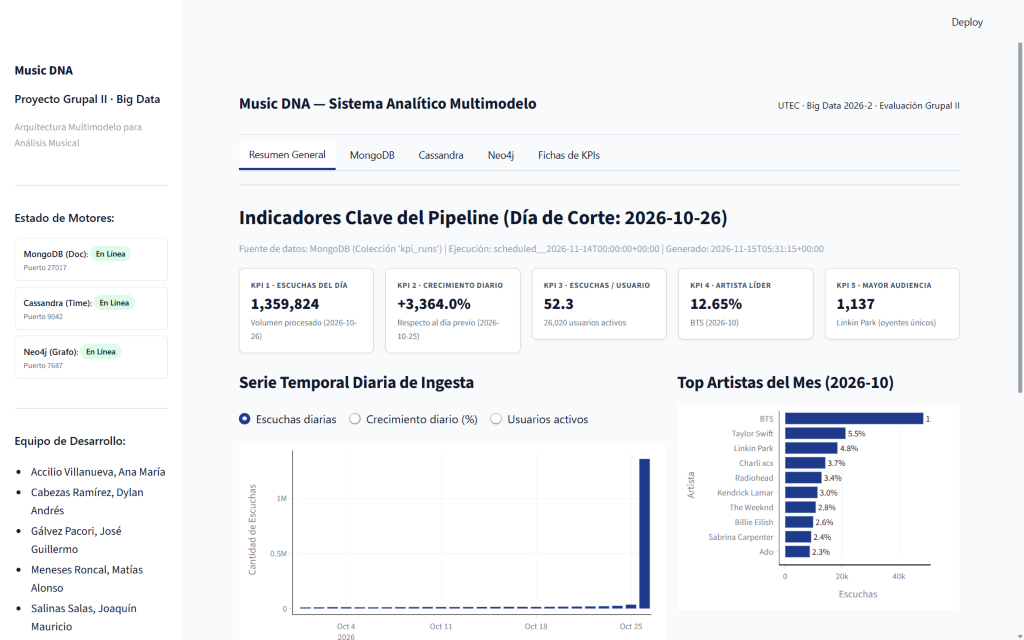
\includegraphics[width=\textwidth]{figuras/dashboard_general.png}
\nota{La interfaz muestra el diagnóstico de los tres motores, las cinco tarjetas de KPIs para el día de referencia, la serie diaria con selector de métrica y el top de artistas de octubre.}
\end{figure}

El panel central integra un selector interactivo que permite alternar la serie temporal de los últimos 30 días entre volumen diario, tasa de crecimiento interdiario y usuarios activos. A la derecha, un gráfico de barras horizontales desglosa la participación porcentual del top de artistas del mes de referencia, evidenciando el liderazgo de BTS frente a Taylor Swift, Linkin Park y Charli xcx.

En la sección inferior se despliegan las métricas de seguimiento de la carga incremental (4\,000\,000 de documentos en MongoDB, 10 lotes y 4\,855\,809 escuchas en Cassandra, modularidad ponderada de 0,7825 en Neo4j) y la tabla comparativa que refleja cómo evolucionan los indicadores a través de las corridas del DAG registradas en la colección \code{kpi_runs}.

\subsection{Vistas especializadas de persistencia}

La figura~\ref{fig:dashboard-cassandra} ilustra la vista analítica especializada en Cassandra. En ella se combinan gráficos interactivos desarrollados en Plotly que contrastan la evolución mensual de reproducciones con la distribución horaria de actividad en horario UTC. El análisis horario evidencia un pico sostenido de consumo entre las 16:00 y las 20:00 UTC (alcanzando 389\,000 escuchas a las 18:00 UTC), representativo del horario vespertino en Europa y América.

\begin{figure}[H]
\caption{Vista especializada de Cassandra: series temporales y distribución horaria}
\label{fig:dashboard-cassandra}
\centering
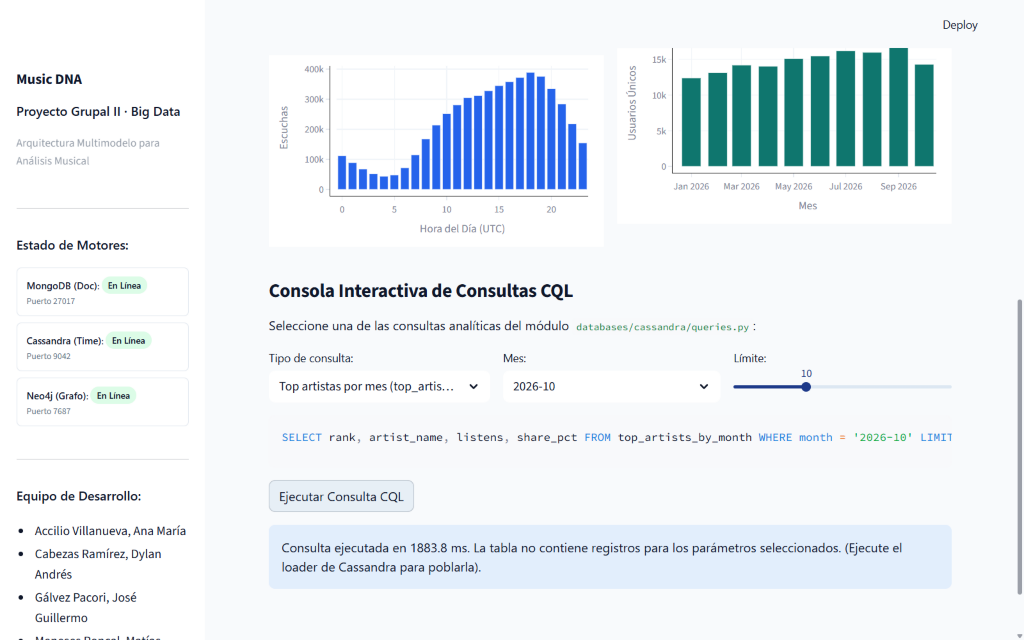
\includegraphics[width=\textwidth]{figuras/dashboard_cassandra.png}
\nota{Evolución mensual de reproducciones, distribución horaria agregada en UTC y desglose de la estrategia de particionamiento tabular.}
\end{figure}

En la figura~\ref{fig:dashboard-neo4j} se expone el módulo de análisis de redes y grafos conectado a Neo4j. La tabla superior resume las comunidades musicales detectadas por el algoritmo de Louvain, complementada por un gráfico de barras de audiencia por clúster. La sección inferior incorpora un motor interactivo de recomendaciones explicables que permite seleccionar un artista canónico y visualizar recomendaciones ponderadas por el coeficiente de similitud de Jaccard y su comunidad de pertenencia.

\begin{figure}[H]
\caption{Vista especializada de Neo4j: comunidades de Louvain y recomendador explicable}
\label{fig:dashboard-neo4j}
\centering
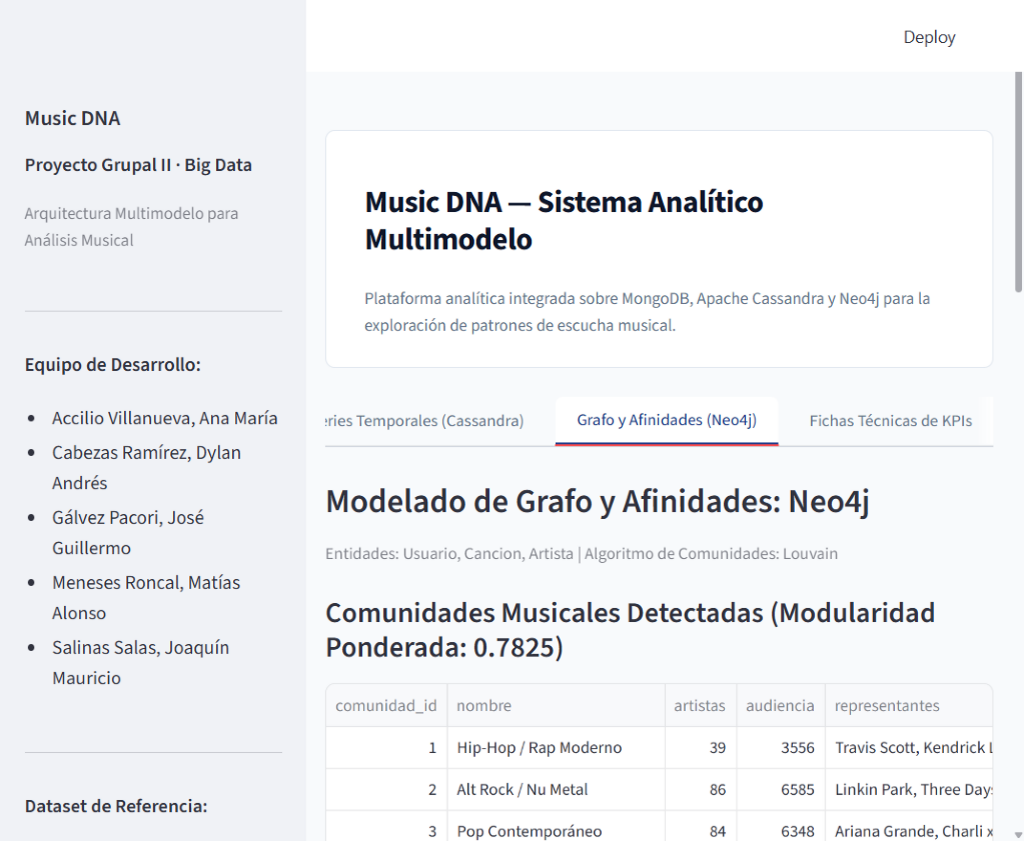
\includegraphics[width=\textwidth]{figuras/dashboard_neo4j.png}
\nota{Comunidades del grafo, identificación de artistas puente y sistema de recomendación explicable con coeficientes de Jaccard.}
\end{figure}

Por último, la figura~\ref{fig:dashboard-kpis} presenta el módulo de fichas técnicas de los KPIs, diseñado específicamente para cumplir los criterios de rigor metodológico exigidos en el curso, exponiendo las fórmulas matemáticas KaTeX y la tabla comparativa de los valores calculados a lo largo de las distintas corridas de Airflow.

\begin{figure}[H]
\caption{Módulo de fichas técnicas formales de los 5 KPIs}
\label{fig:dashboard-kpis}
\centering
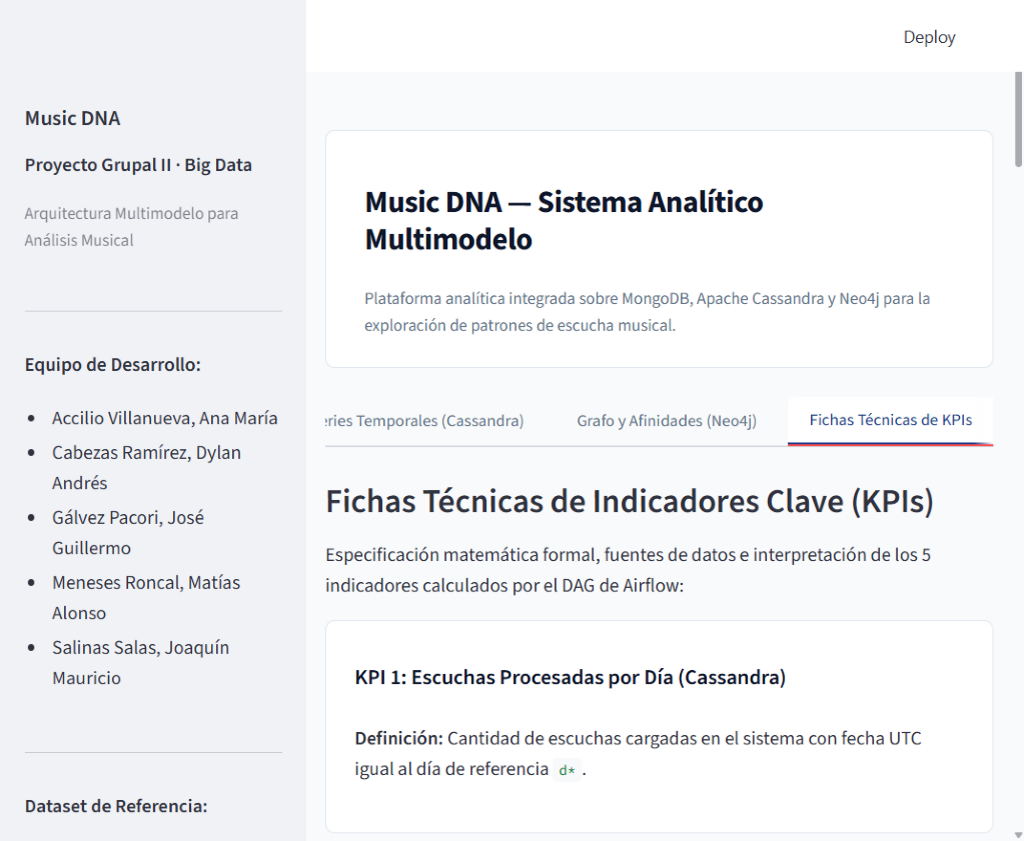
\includegraphics[width=\textwidth]{figuras/dashboard_kpis.png}
\nota{Fichas técnicas con fórmulas matemáticas en KaTeX, fuentes de datos, interpretación y tabla comparativa por lotes de Airflow.}
\end{figure}

\section{Conclusiones}
\label{cap:conclusiones}

El proyecto construyó una arquitectura multimodelo completa sobre un volcado real de ListenBrainz de 4\,855\,809 escuchas: MongoDB con los documentos originales, Cassandra con la serie temporal y los agregados, Neo4j con el grafo de relaciones y un DAG de Airflow que mantiene las tres bases a partir de la misma fuente y calcula cinco indicadores. Todo se levanta con un solo \code{docker-compose.yml}.

\subsection{Aprendizajes}

Aprendimos que el modelo de datos se diseña a partir de las consultas. En Cassandra eso es explícito: una tabla por consulta, particiones por usuario y mes para que ninguna crezca sin límite y el ranking guardado como clustering porque es la única forma de que Cassandra lo devuelva ordenado. A cambio, las consultas de Cassandra tardan entre 6 y 16~ms sobre millones de filas. En Neo4j el mismo criterio llevó a agregar las escuchas en relaciones con cantidad y proporción, que redujeron 4,86 millones de eventos a 1,79 millones de relaciones usuario--canción y dejaron en el grafo exactamente lo que necesitan las recomendaciones.

En un pipeline que se reintenta, la idempotencia importa más que la velocidad. Las tres cargas se pueden repetir sin duplicar datos por razones distintas: huellas SHA-256 y checkpoint en MongoDB, ids deterministas y registro de lotes en Cassandra, \texttt{MERGE} y estado del lote en Neo4j. En Cassandra esto incluso obligó a abandonar los counters, que suman dos veces si un lote se repite, y a recalcular los agregados en cada carga.

También vimos que hay que conocer el dato antes de interpretarlo. Un incremental describe la ingesta, no la escucha: hay escuchas fechadas en 2005 enviadas en 2026, el 26 de octubre concentra el 28~\% del archivo y el volcado se corta el 27 a las 00:01. Sin esa lectura, el crecimiento de $+3\,364$~\% o la participación de BTS parecerían hallazgos sobre los oyentes, cuando son efectos de cómo llegaron los datos.

\subsection{Trabajo futuro}

Como siguiente paso, \code{extraer_datos} puede descargar el siguiente incremental publicado por ListenBrainz, Neo4j puede cargarse de forma incremental, Cassandra puede recalcular solo los días y meses que toca cada lote, y los artistas pueden normalizarse con los identificadores de MusicBrainz.

\subsection{Repositorio y video}

El código fuente completo (loaders, scripts de creación de las bases, DAG de Airflow y dashboard) está en el repositorio \repolink. El video demostrativo (carpeta de Google Drive) está disponible en \videolink.


\begin{thebibliography}{99}
\addcontentsline{toc}{chapter}{Referencias}

\bibitem{listenbrainz-data}
MetaBrainz Foundation. \emph{ListenBrainz -- Data Downloads}.
\url{https://listenbrainz.org/data/}

\bibitem{listenbrainz-dumps}
MetaBrainz Foundation. \emph{ListenBrainz Data Dumps}. Documentación de ListenBrainz.
\url{https://listenbrainz.readthedocs.io/en/latest/users/listenbrainz-dumps.html}

\bibitem{listenbrainz-json}
MetaBrainz Foundation. \emph{ListenBrainz JSON Documentation}.
\url{https://listenbrainz.readthedocs.io/en/latest/users/json.html}

\bibitem{incremental-2746}
MetaBrainz Foundation. Directorio del incremental 2746 (27 de octubre de 2026).
\url{https://data.metabrainz.org/pub/musicbrainz/listenbrainz/incremental/listenbrainz-dump-2746-20261027-000003-incremental/}

\bibitem{mongodb}
MongoDB, Inc. \emph{MongoDB Manual}.
\url{https://www.mongodb.com/docs/manual/}

\bibitem{cassandra}
The Apache Software Foundation. \emph{Apache Cassandra Documentation}.
\url{https://cassandra.apache.org/doc/latest/}

\bibitem{neo4j}
Neo4j, Inc. \emph{Neo4j Cypher Manual}.
\url{https://neo4j.com/docs/cypher-manual/current/}

\bibitem{airflow}
The Apache Software Foundation. \emph{Apache Airflow Documentation}, versión 2.10.
\url{https://airflow.apache.org/docs/apache-airflow/2.10.5/}

\bibitem{streamlit}
Snowflake Inc. \emph{Streamlit Documentation}.
\url{https://docs.streamlit.io/}

\bibitem{networkx}
NetworkX Developers. \emph{NetworkX: Louvain Community Detection}.
\url{https://networkx.org/documentation/stable/reference/algorithms/generated/networkx.algorithms.community.louvain.louvain_communities.html}

\end{thebibliography}

\end{document}
